%%%%%%%%%%%%%%%%%%%%%%%%%%%%%%%%%%%%%%%%%%%%%%%%%%%%%%%%%%%%%%%%%%%%%%%%
\clearpage
\section{Cylindrical objects}


%%%%%%%%%%%%%%%%%%%%%%%%%%%%%%%%%%%%%%%%%%%%%%%%%%%%%%%%%%%%%%%%%%%%%%%%%

%\clearpage
\subsection{Helical structures} ~\\
Several approaches for describing the small angle scattering signal from randomly oriented helical structures have been published.
In \cite{Franklin1956,Puigjaner1974} a model of a double helix with a round cross section for each strand has been developed. For a fanlike cross section of a double helix a solution has been given by \cite{Schmidt1970,Pringle1971}. Fukuda et al.\ \cite{Fukuda2002} have extended the model to an arbitrary shaped cross section. In a model developed by Lebedev et al.\ \cite{Lebedev2003} it is assumed, that beads are arranged on a helical path assuming a single strand. In all models the helix is straight and its length dimension is large compared to all other characteristic length of the helix.
In \cite{Benham1980} a solution of a single helical strand which can have a secondary coiling has been described. In this paper the cross section of the helical strand is assumed to be infinitesimal thin.

~\\
\subsubsection{Fanlike helix} ~\\
Double helices with a fanlike cross section in the plane perpendicular to the helix axis have been described by by Schmidt and Pringle \cite{Schmidt1970,Pringle1971}. The model has been generalized by Fakuda et al.\ \cite{Fukuda2002} for an arbitrarily shaped cross section and by Teixeira et al.\ \cite{Teixeira2010} to a multi radial shell with fanlike cross section.
\begin{figure}[htb]
\begin{center}
  \subfigure[top on view]{\label{fig:fanhelixside1}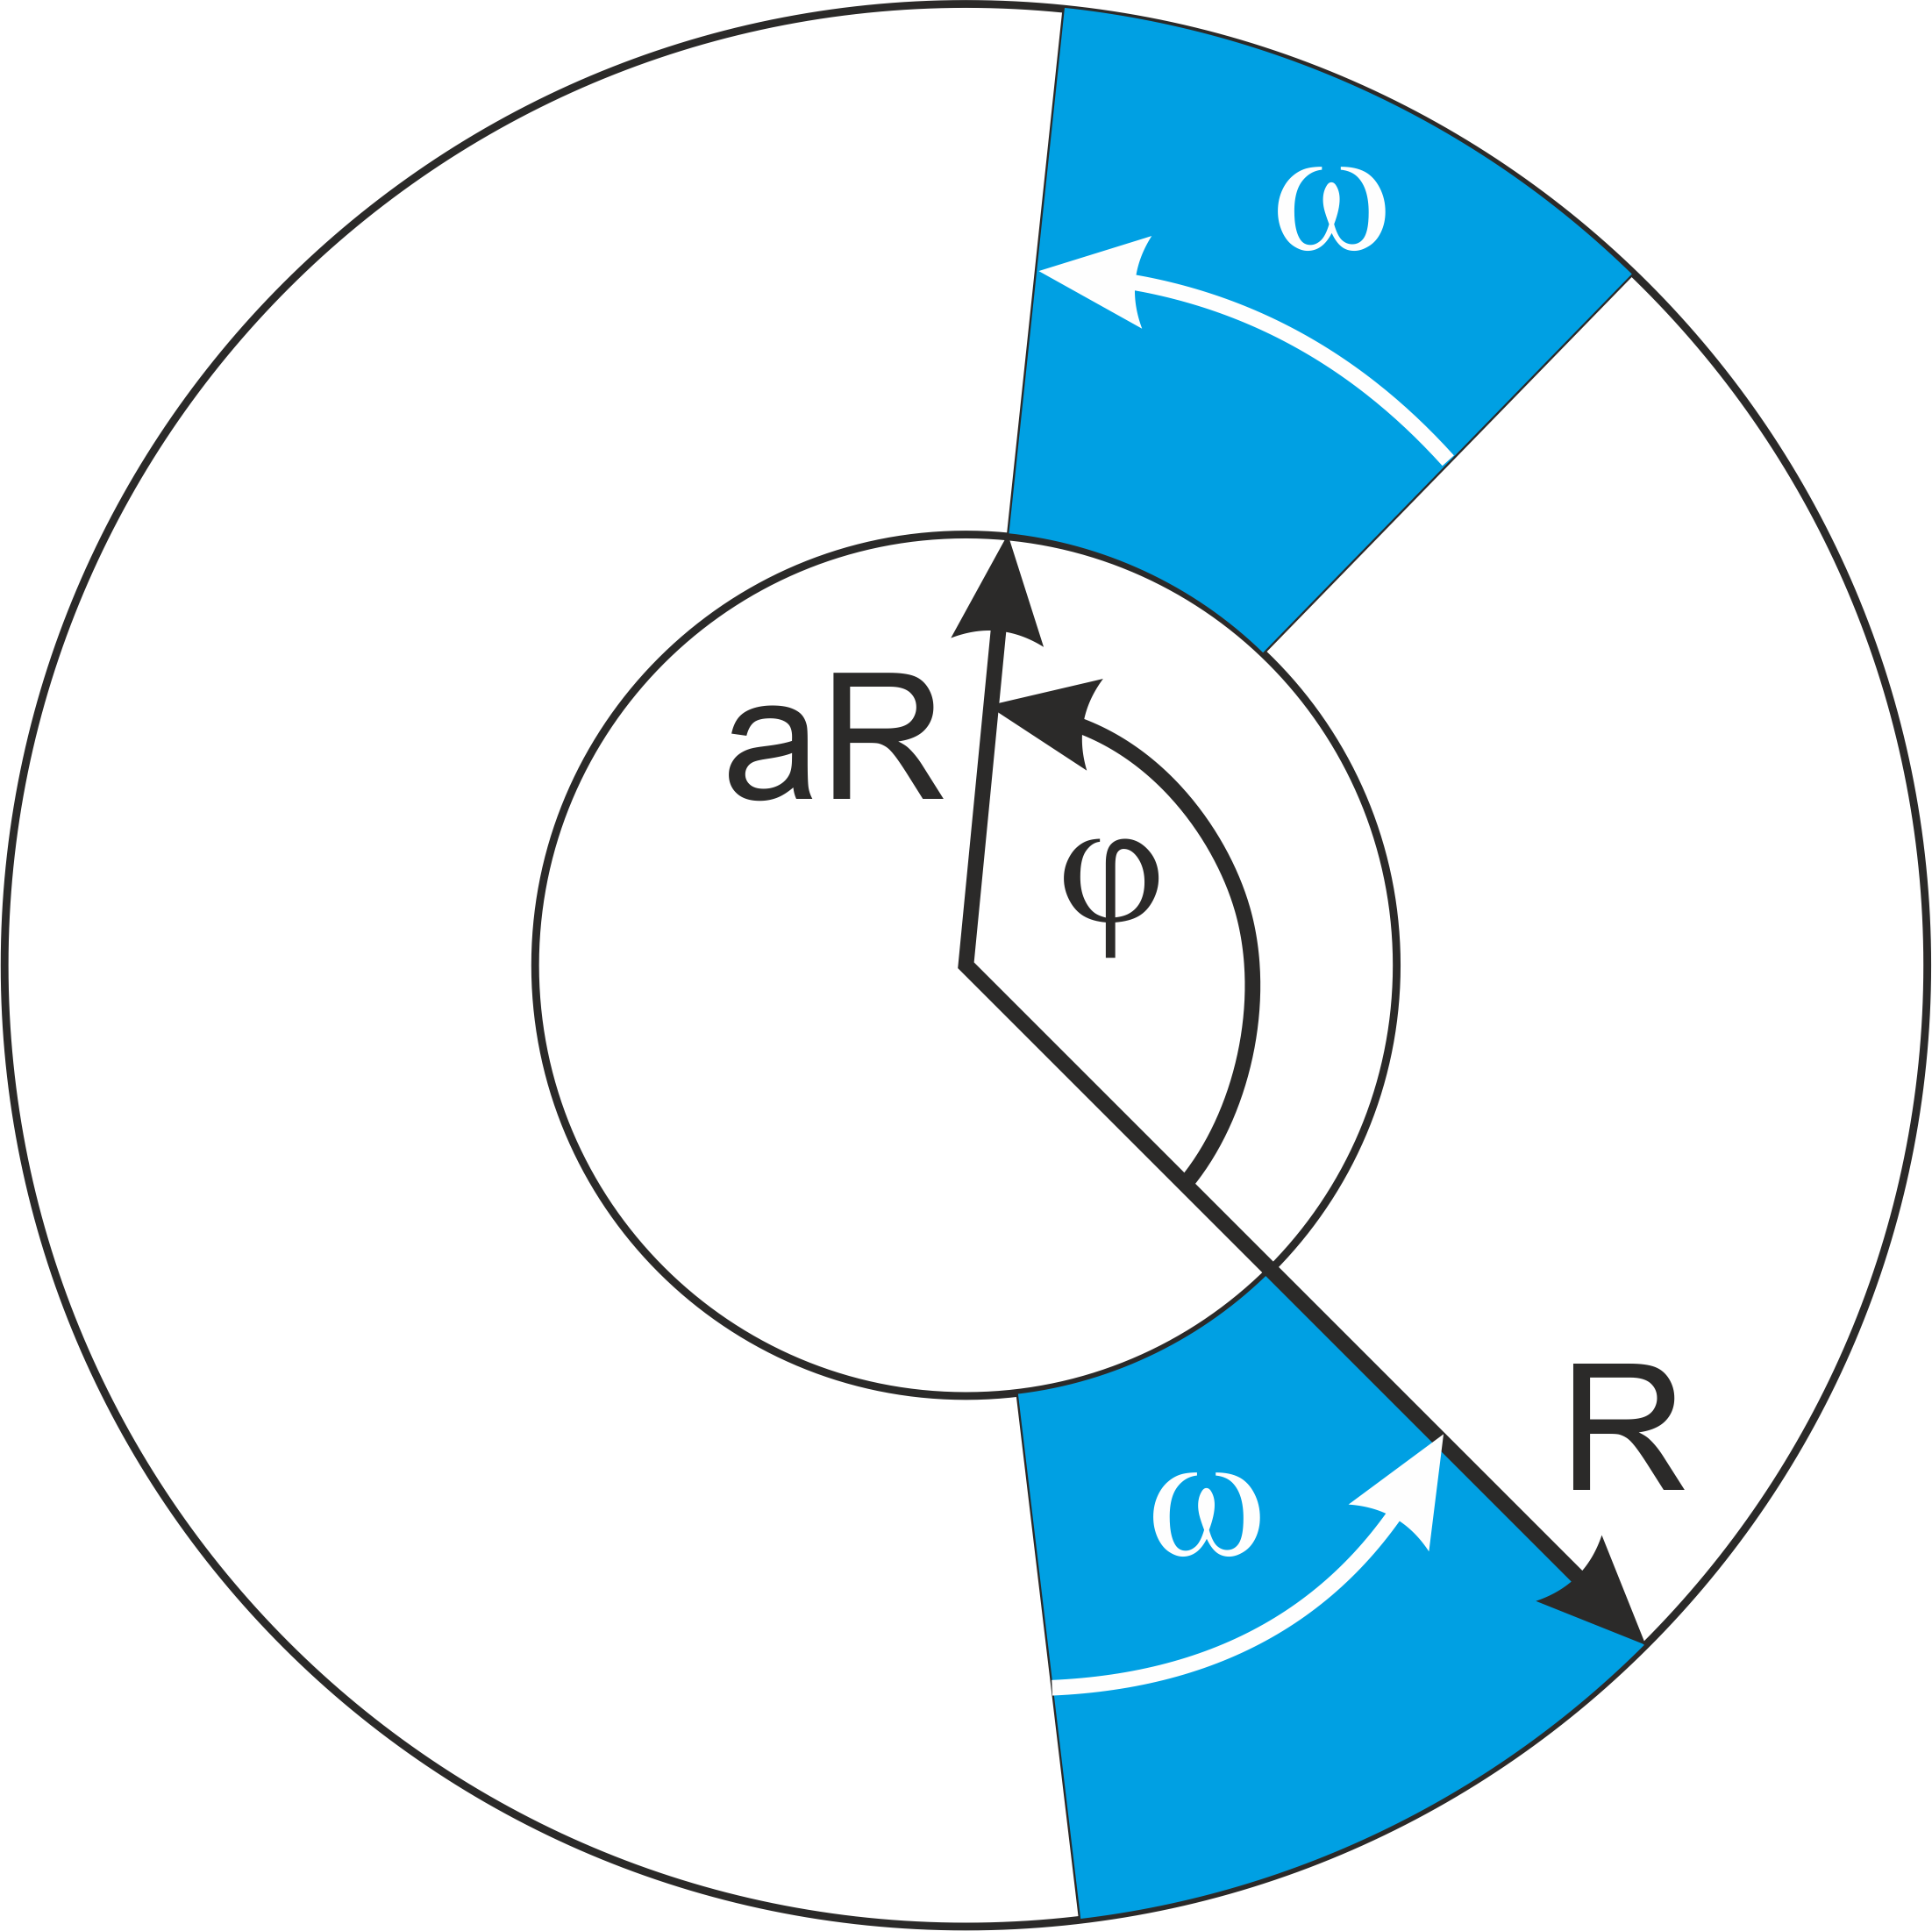
\includegraphics[width=0.45\textwidth]{../images/form_factor/cylindrical_obj/fanlike_helicesXS.png}}
\hfill
  \subfigure[side view]{\label{fig:fanhelixside2}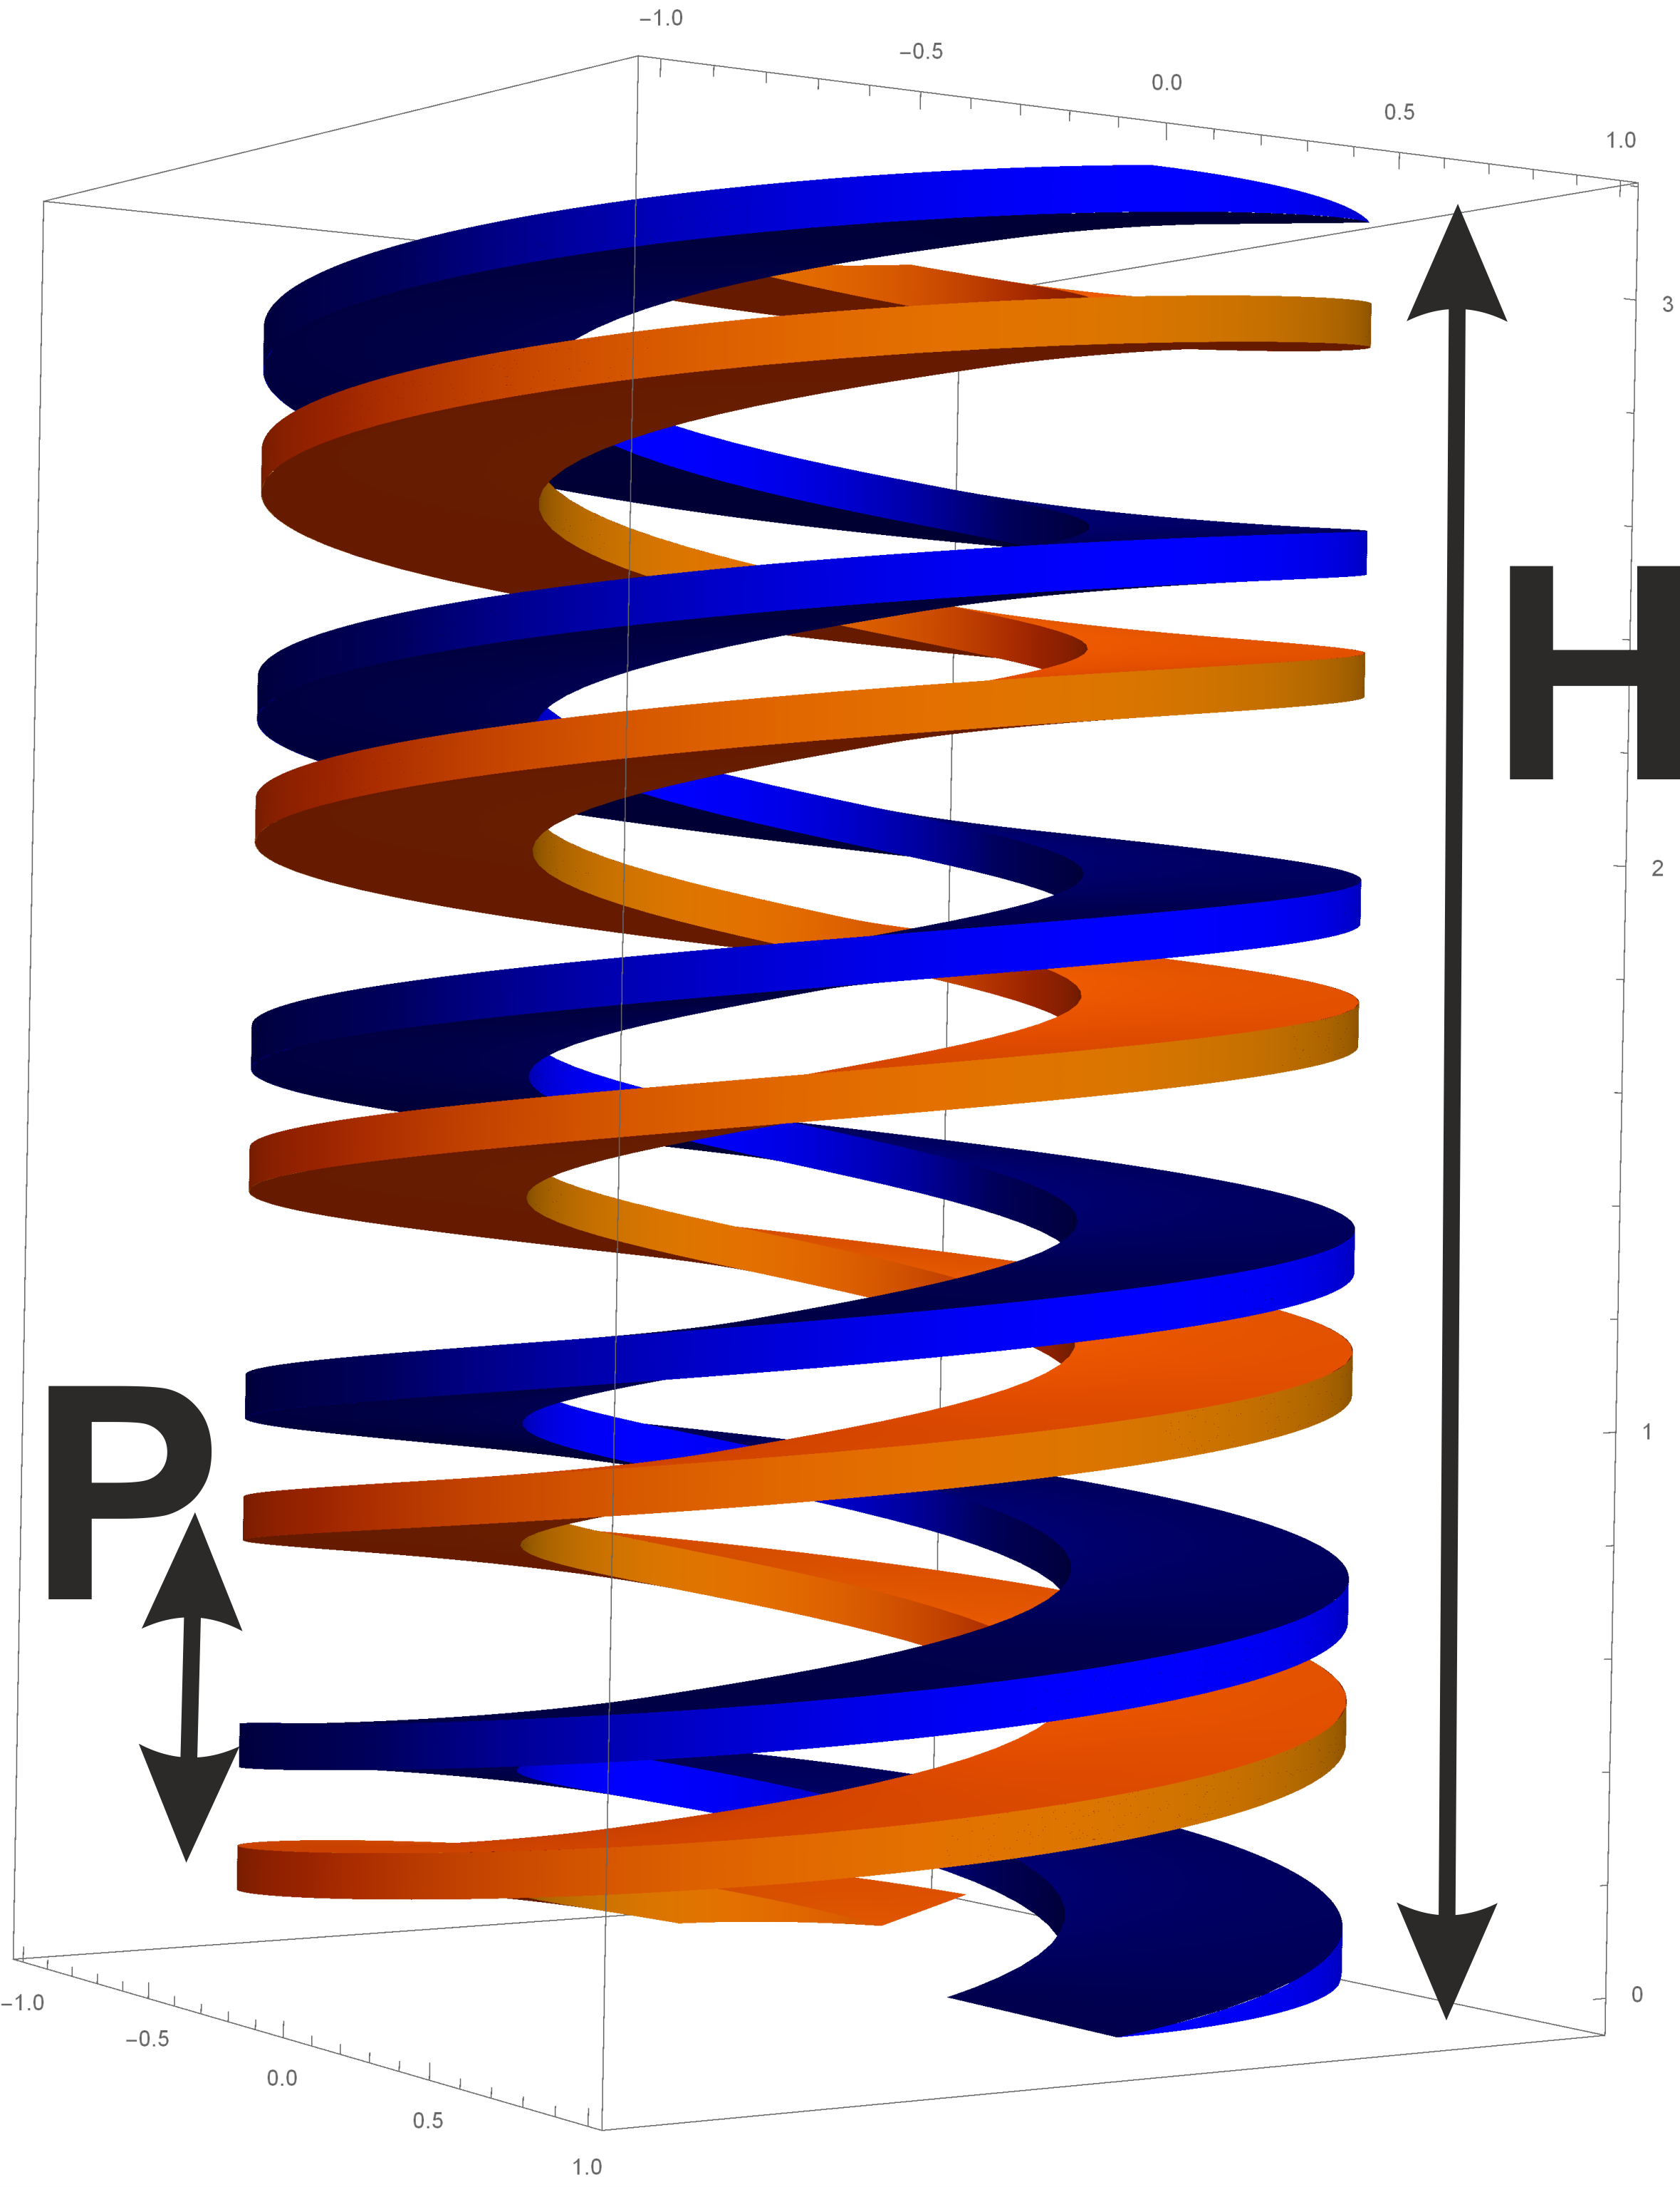
\includegraphics[width=0.45\textwidth]{../images/form_factor/cylindrical_obj/fanlike_helices3D.png}}
\end{center}
\caption{Double helix with strands of round cross sections.} \label{fig:fanhelix}
\end{figure}

\begin{align}
\begin{split}
I(Q) &= P_\text{rod}(Q,H) \left(\left(\eta_\text{h}-\eta_\text{solv}\right)\omega R^2\left(1-a^2\right)\right)^2 \\
&\times \sum_{n=0}^\infty \epsilon_n \left( \cos(n\varphi/2) \frac{\sin(n\omega/2)}{n\omega/2} g_n\left(Q,R,a\right)\right)^2
\end{split} \\
g_n\left(Q,R,a\right) &= \frac{2}{R^2\left(1-a^2\right)} \int_{aR}^R r' J_n\left(Qr'\left(1-q_n^2\right)\right)\mathrm{d}r' \\
q_n &=
\begin{cases}
\begin{array}{rcl}
\frac{2\pi n}{QP} & \text{for} & Q\geq \frac{2\pi n}{P}\\
1 & \text{for} & Q < \frac{2\pi n}{P}
\end{array}
\end{cases} \\
P_\text{rod}(Q,H) &= H^2 \left(2\frac{\mathrm{Si}(QH)}{(QH)}-\left(\frac{\sin(QH/2)}{QH/2}\right)^2\right)
\end{align}
with $\epsilon_n=1$ for $n=0$ and $\epsilon_n=2$ for $n\geq 1$.

The sum converges very fast and for small $Q$-values the first few terms are already sufficient. However, {\tt SASfit} is continuing the sum until the relative change of the sum is less than $10^{-10}$.

The forward scattering of the model is normalized to the squared scattering length density contrast and squared total volume of the helix so that
\begin{align}
I(Q=0) &= \left(H\left(\eta_\text{h}-\eta_\text{solv}\right)\omega R^2\left(1-a^2\right)\right)^2
\end{align}

\vspace{5mm}

\underline{Input Parameters for model \texttt{fanlike helix}:}\\
\begin{description}
\item[\texttt{R}] external helix radius $R$
\item[\texttt{a}] inner helix radius $aR$, with $0\leq a\leq 1$
\item[\texttt{omega}] angular of the sector of material $\omega$
\item[\texttt{phi}] angle between the two sectors of matrerial $\varphi$
\item[\texttt{dummy}] not used
\item[\texttt{P}] height of one helix period $P$
\item[\texttt{H}] total length of helix $H$
\item[\texttt{eta\_h}] scattering length density of helix $\eta_\text{h}$
\item[\texttt{dummy}] not used
\item[\texttt{eta\_solv}] scattering length density of solvent $\eta_\text{solv}$
\end{description}

\noindent\underline{Note:}
\begin{itemize}
\item The helix is assumed to be stiff and long so that it scattering intensity can be factorized in a cross-section contribution and a shape contribution, whereas the shape contribution can be described by an infinitesimal thin rod of length $H$.
\item $R$, $P$, and $H$ are only physical for values larger than 0.
\item The model is an approximation for the limit $H \gg P$ and $H \gg R$.
\item $0\leq a\leq 1$
\end{itemize}

\begin{figure}[htb]
\begin{center}
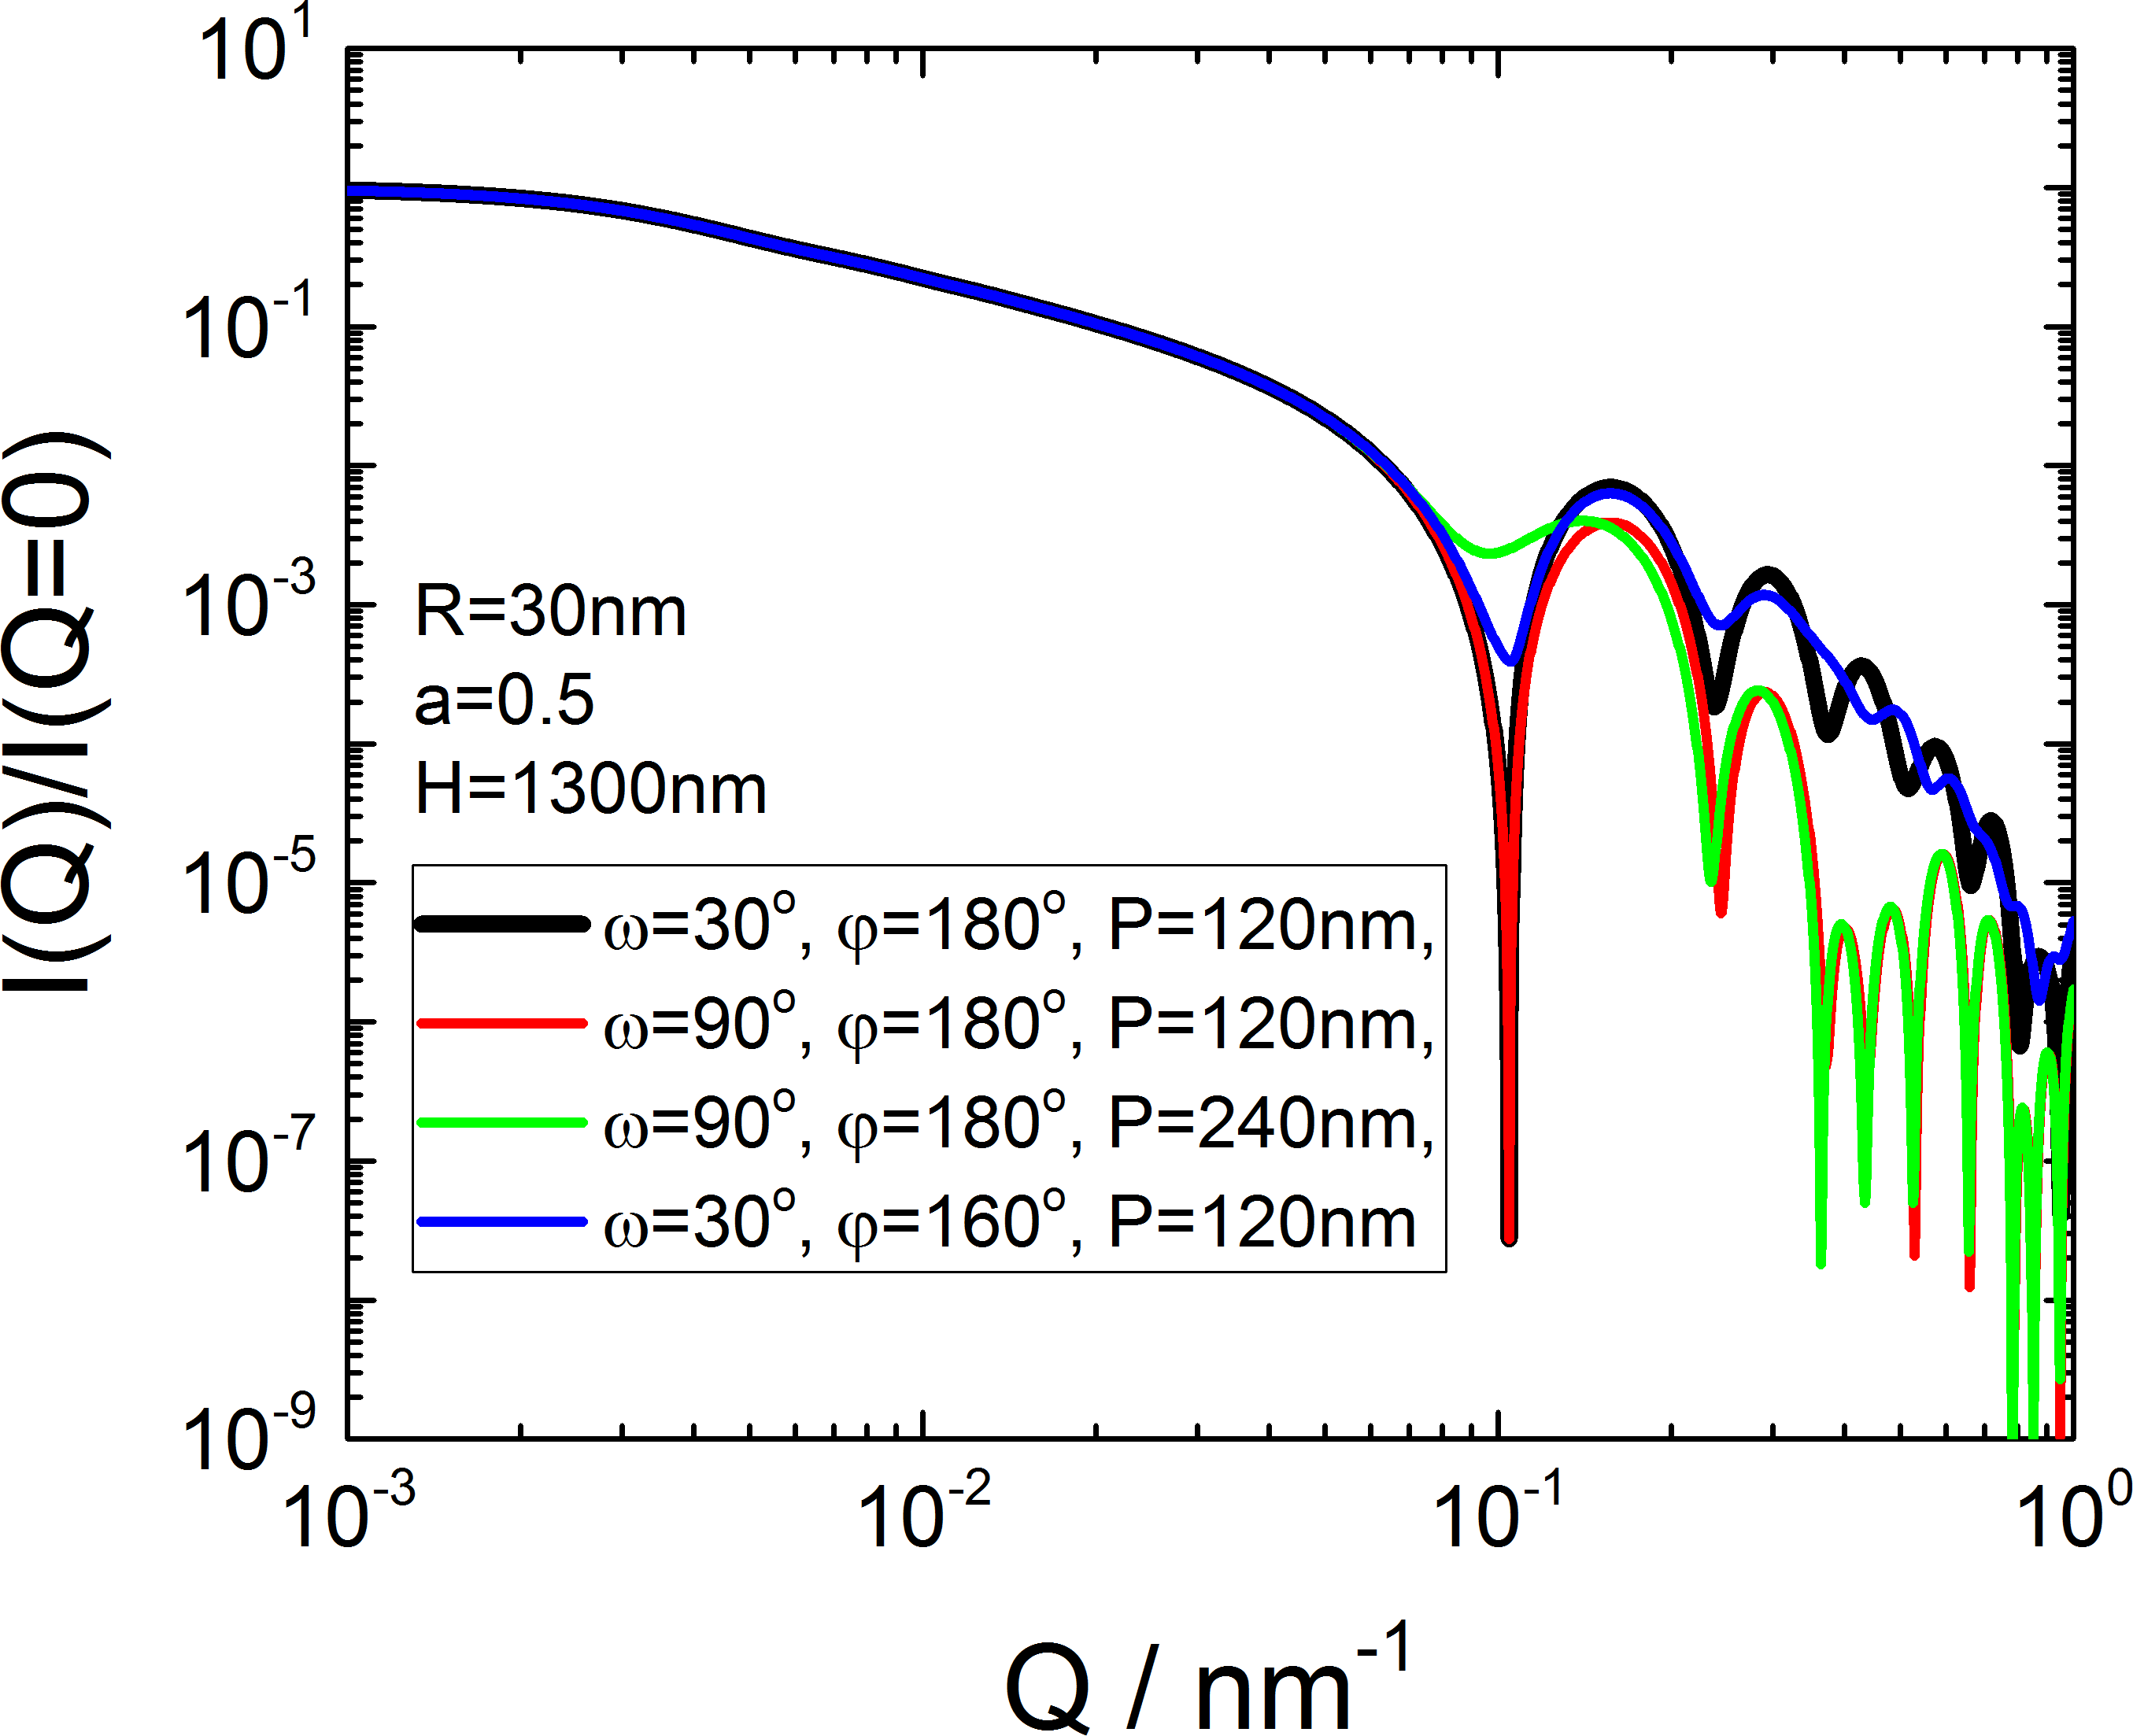
\includegraphics[width=0.7\textwidth]{../images/form_factor/cylindrical_obj/helix_fanlike_IQ.png}
\end{center}
\caption{Normalized scattering curves of fanlike helices.}
\label{fig:helixfanlikeIQ}
\end{figure}

%\phantom{.}~\\
\newpage
\subsubsection{Helix with round cross-section} ~\\
Originally Franklin et al.\ \cite{Franklin1956} and Puigjaner et al.\ \cite{Puigjaner1974} have given the form factor of a cylinder with a groove of a double helix shape of round cross section. Fukada \cite{Fukuda2002} is discussing the form factor of the random oriented double helices alone, but with arbitrary cross-sections.
\begin{figure}[htb]
\begin{center}
  \subfigure[top on view]{\label{fig:roundhelix1}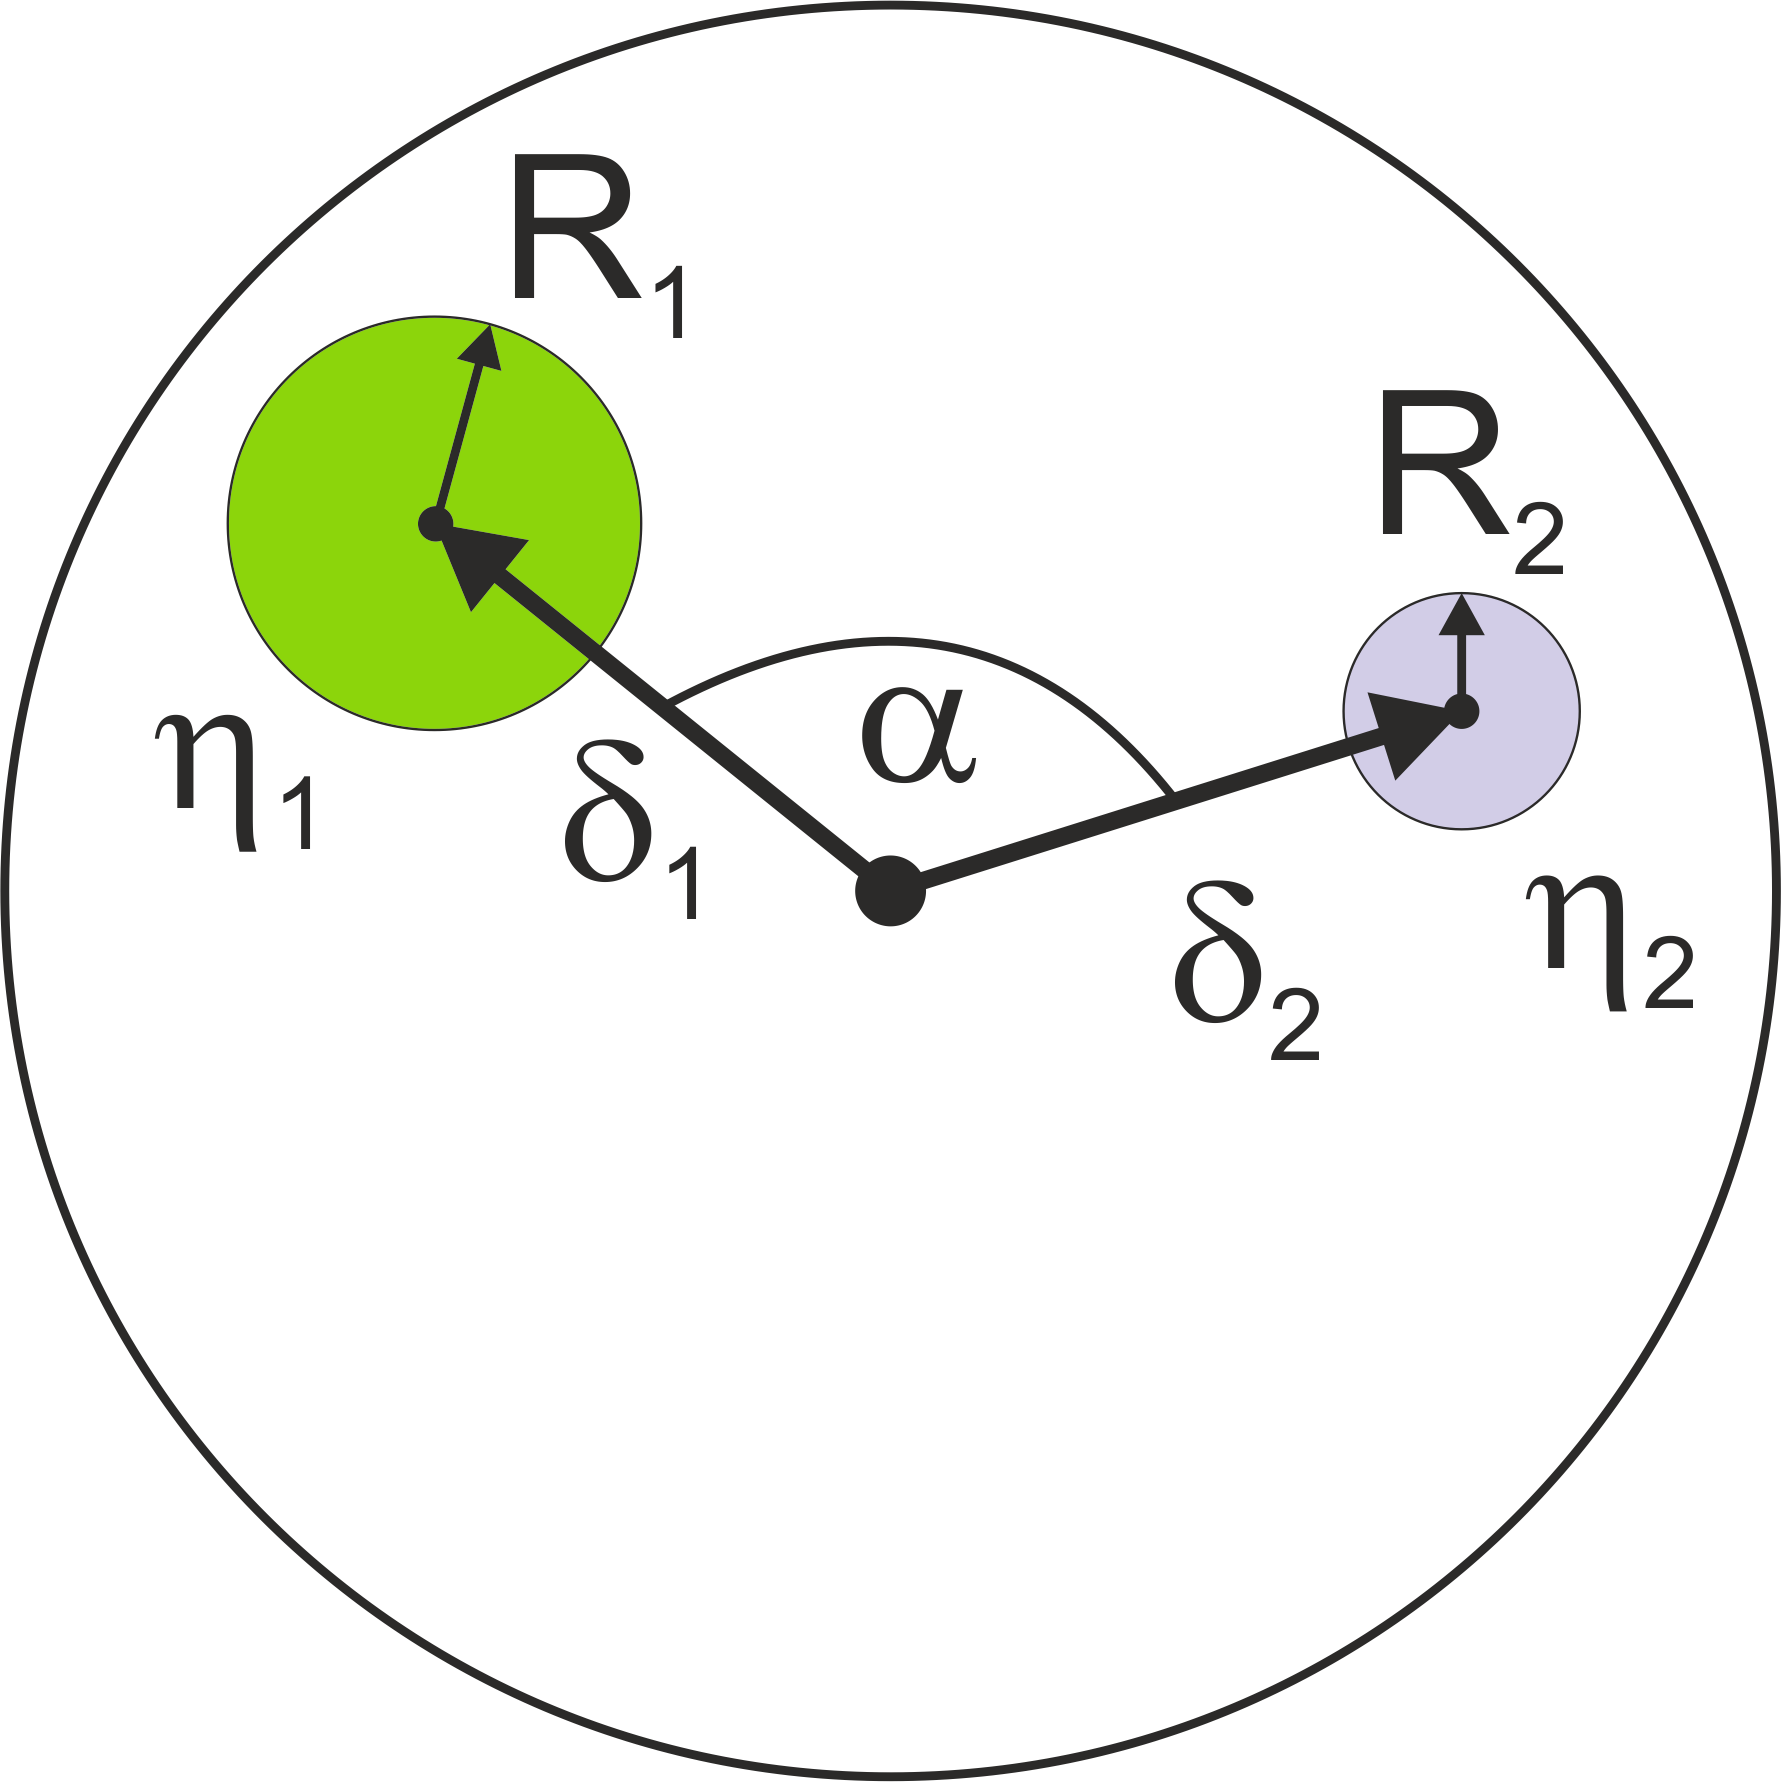
\includegraphics[width=0.45\textwidth]{../images/form_factor/cylindrical_obj/roundhelices1.png}}
\hfill
  \subfigure[side view]{\label{fig:roundhelix2}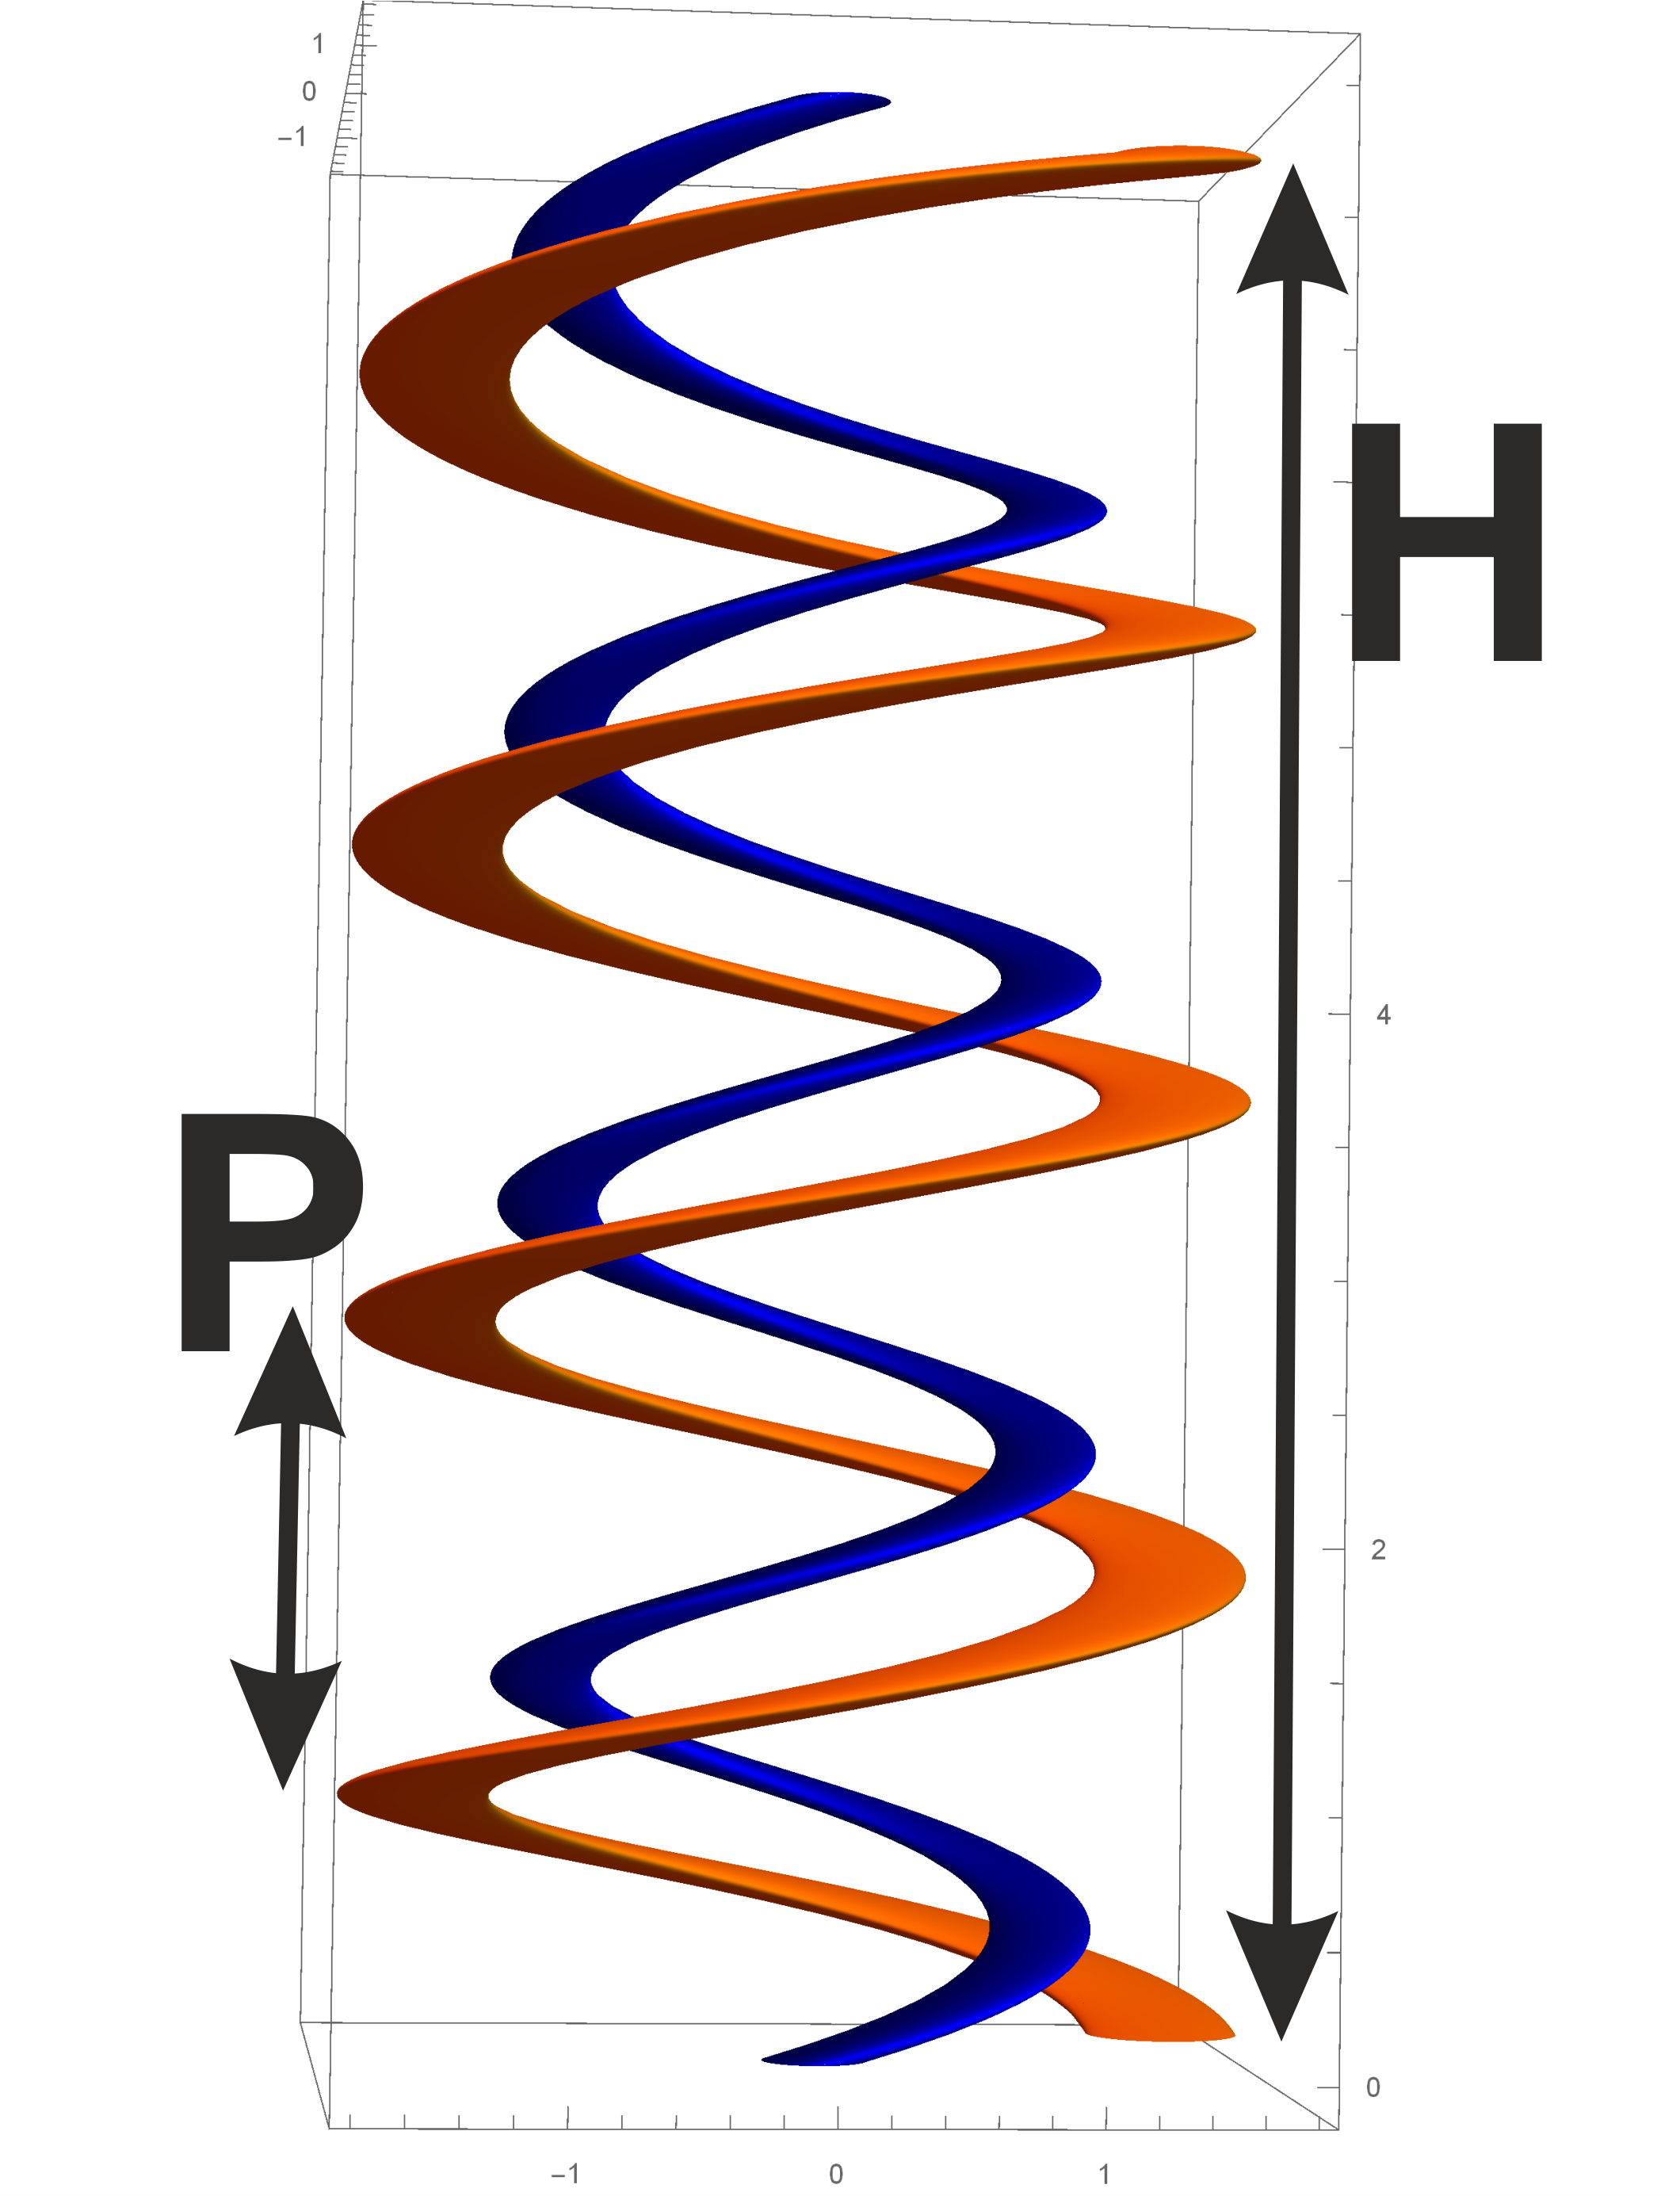
\includegraphics[width=0.45\textwidth]{../images/form_factor/cylindrical_obj/round_helices3D.png}}
\end{center}
\caption{Double helix with strands of round cross sections. The cross-sections are round in the plane perpendicular to the helix axis.} \label{fig:roundhelix}
\end{figure}

\begin{align}
I(Q) &= P_\text{rod}(Q,H) \sum_{n=0}^{\infty} \epsilon_n \left( A_{1n}^2 + A_{2n}^2+2A_{1n}A_{2n}\cos n\alpha\right)
\label{eq:roundhelix1}
\end{align}
where
\begin{align}
A_{in} &= J_n\left(\delta_i Q_\perp\right) \pi R_i^2 \left(\eta_i-\eta_\mathrm{solv}\right)\frac{2J_1\left(R_i Q_\perp\right)}{R_i Q_\perp} \\
Q_\perp^2 &= Q^2-\left[\frac{2\pi n}{P}\right]^2
\end{align}
with $\epsilon_j=1$ for $j=0$ and $\epsilon_j=2$ for $j\geq 1$. Furthermore $R_1$ and $R_2$ are the radii of the round helical strands.
$\delta_1$ and $\delta_2$ are the distances of the strands to the helix axis.
The pitch of the helix is denoted by $P$, whereas $\alpha$ is the angle between the two strands.

The sum converges very fast and for small $Q$-values the first few terms are already sufficient. However, {\tt SASfit} is continuing the sum until the relative change of the sum is less than $10^{-10}$.

The forward scattering of the model is normalized to the squared scattering length density contrast and squared total volume of the helix so that
\begin{align}
I(Q=0) &= H^2\left(\left(\eta_\text{1}-\eta_\text{solv}\right)\pi R_1^2+\left(\eta_\text{2}-\eta_\text{solv}\right)\pi R_2^2\right)^2
\end{align}

\vspace{5mm}

\underline{Input Parameters for model \texttt{helix with round XS}:}\\
\begin{description}
\item[\texttt{R\_1}] radius of first strand thickness $R_1$
\item[\texttt{delta\_1}] distance of first strand to helix axis $\delta_1$
\item[\texttt{R\_2}] radius of second strand thickness $R_2$
\item[\texttt{delta\_2}] distance of second strand to helix axis $\delta_2$
\item[\texttt{alpha}] angle $\alpha$ between the two strands
\item[\texttt{P}] height of one helix period $P$
\item[\texttt{H}] total length of helix $H$
\item[\texttt{eta\_1}] scattering length density of first strand $\eta_1$
\item[\texttt{eta\_2}] scattering length density of second strand $\eta_2$
\item[\texttt{eta\_solv}] scattering length density of solvent $\eta_\text{solv}$
\end{description}

\noindent\underline{Note:}
\begin{itemize}
\item The helix is assumed to be stiff and long so that it scattering intensity can be factorized in a cross-section contribution and a shape contribution, whereas the shape contribution can be described by an infinitesimal thin rod of length $H$.
\item $R_1$, $R_2$, $\delta_1$, $\delta_2$ $P$, and $H$ are only physical for values larger than 0.
\item The model is an approximation for the limit $H \gg P$ and $H \gg R$.
\end{itemize}

\begin{figure}[htb]
\begin{center}
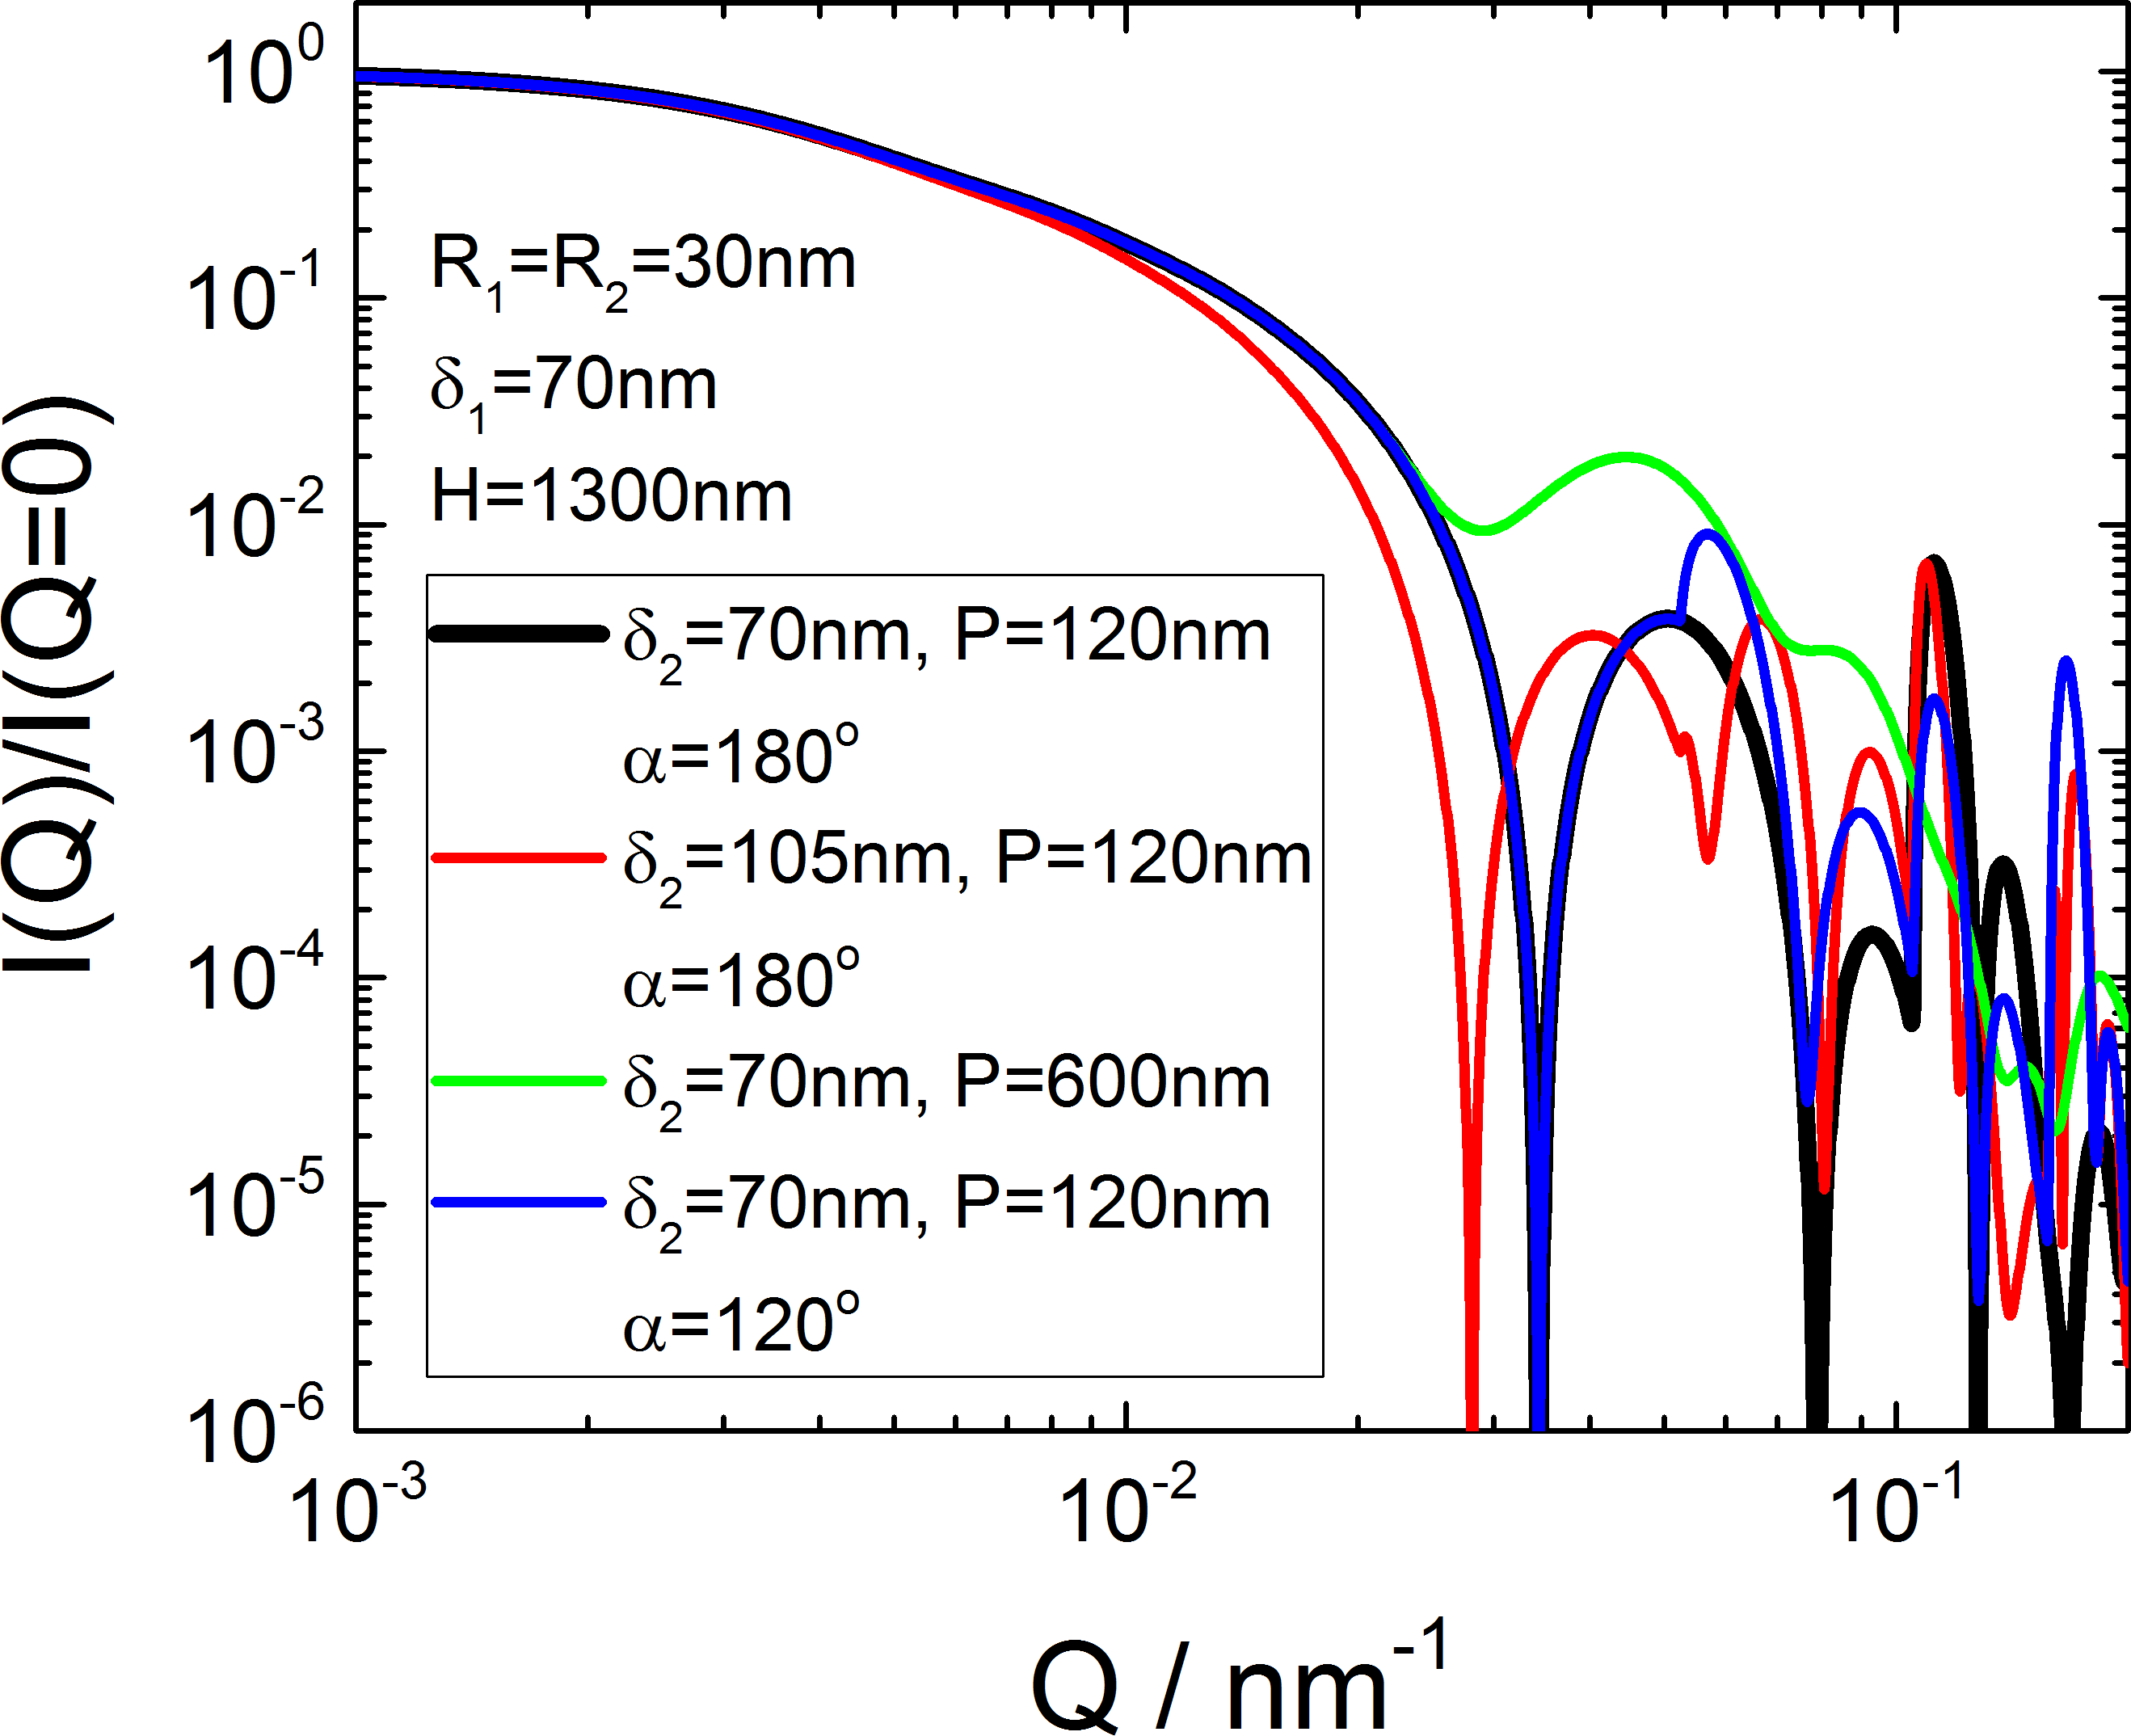
\includegraphics[width=0.7\textwidth]{../images/form_factor/cylindrical_obj/helix_round_IQ.png}
\end{center}
\caption{Normalized scattering curves of helices with round cross sections.}
\label{fig:helixroundIQ}
\end{figure}

%\phantom{.}~\\
\newpage
\subsubsection{Beads model of a single helical strand} ~\\
In this model  \cite{Lebedev2003,Avdeev2013} it is assumed that spherical beads are arranged along the path of a single helical strand. It is the product of the form factor of a sphere and the structure factor described by a helix with an infinitesimal thin single strand.

\begin{figure}[htb]
\begin{center}
  \subfigure[side view]{\label{fig:beadshelixside1}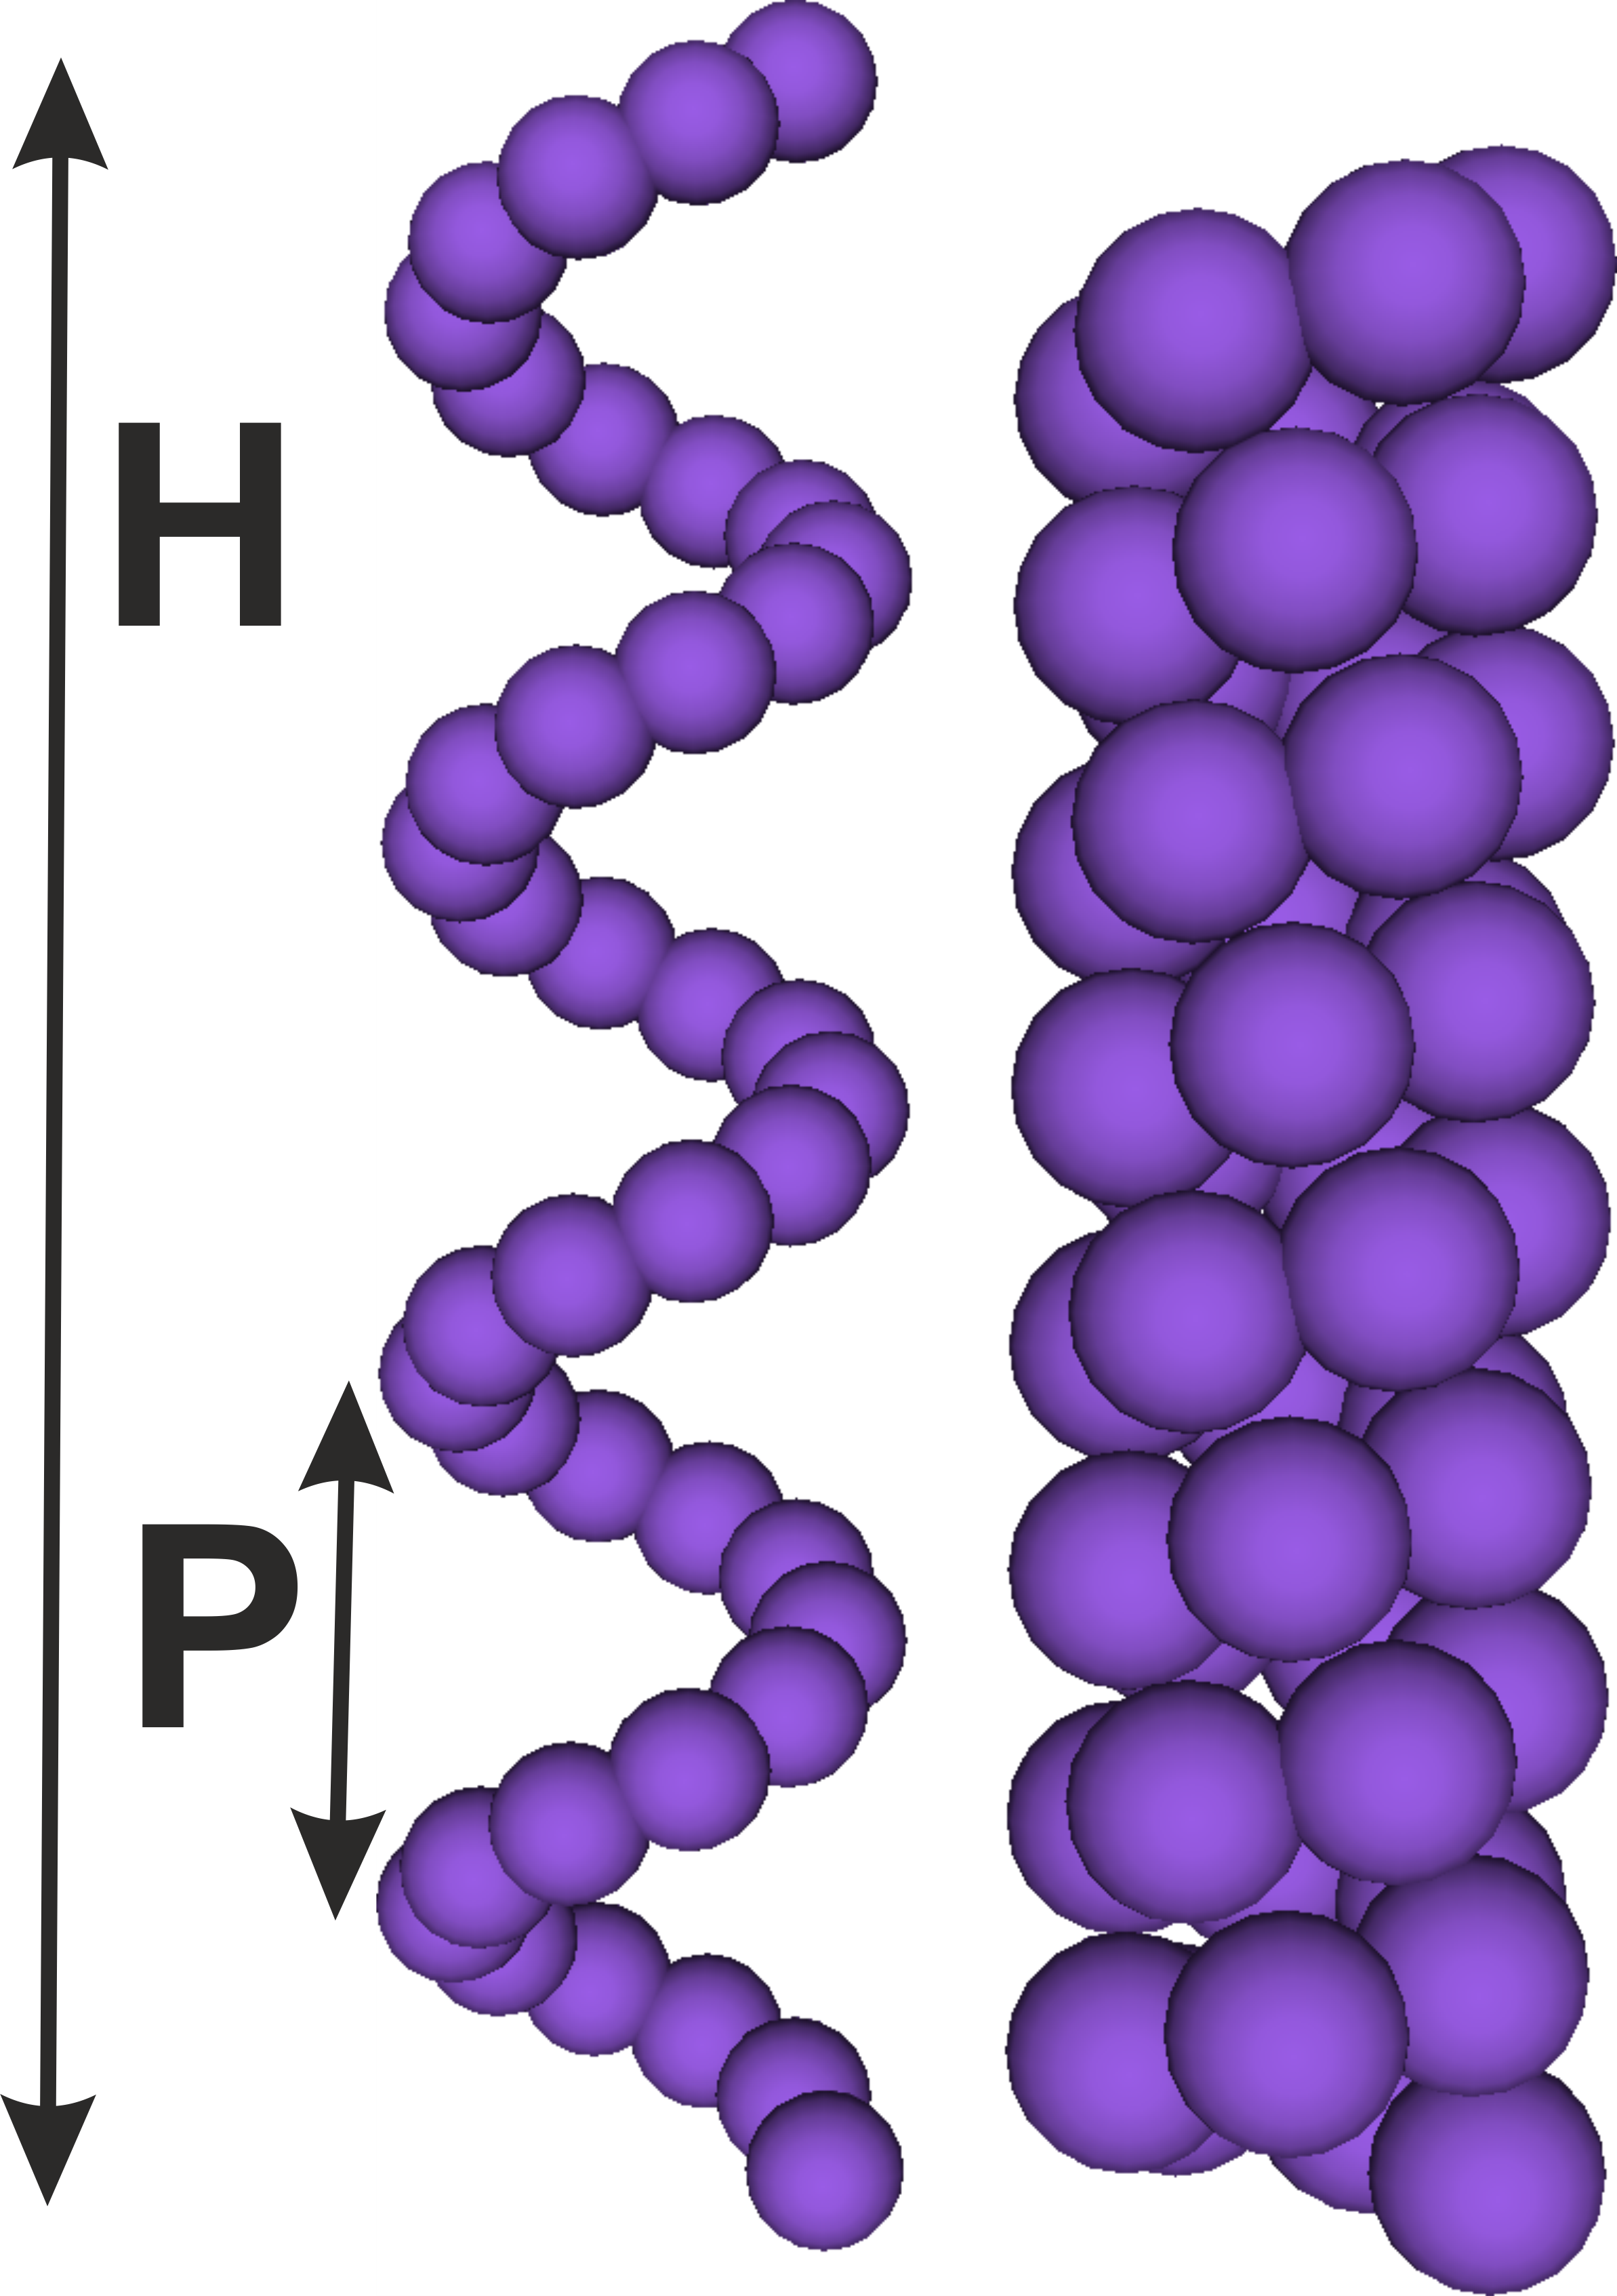
\includegraphics[width=0.4\textwidth]{../images/form_factor/cylindrical_obj/beads_helix_model_1.png}}
\hfill
  \subfigure[top on view]{\label{fig:beadshelixside2}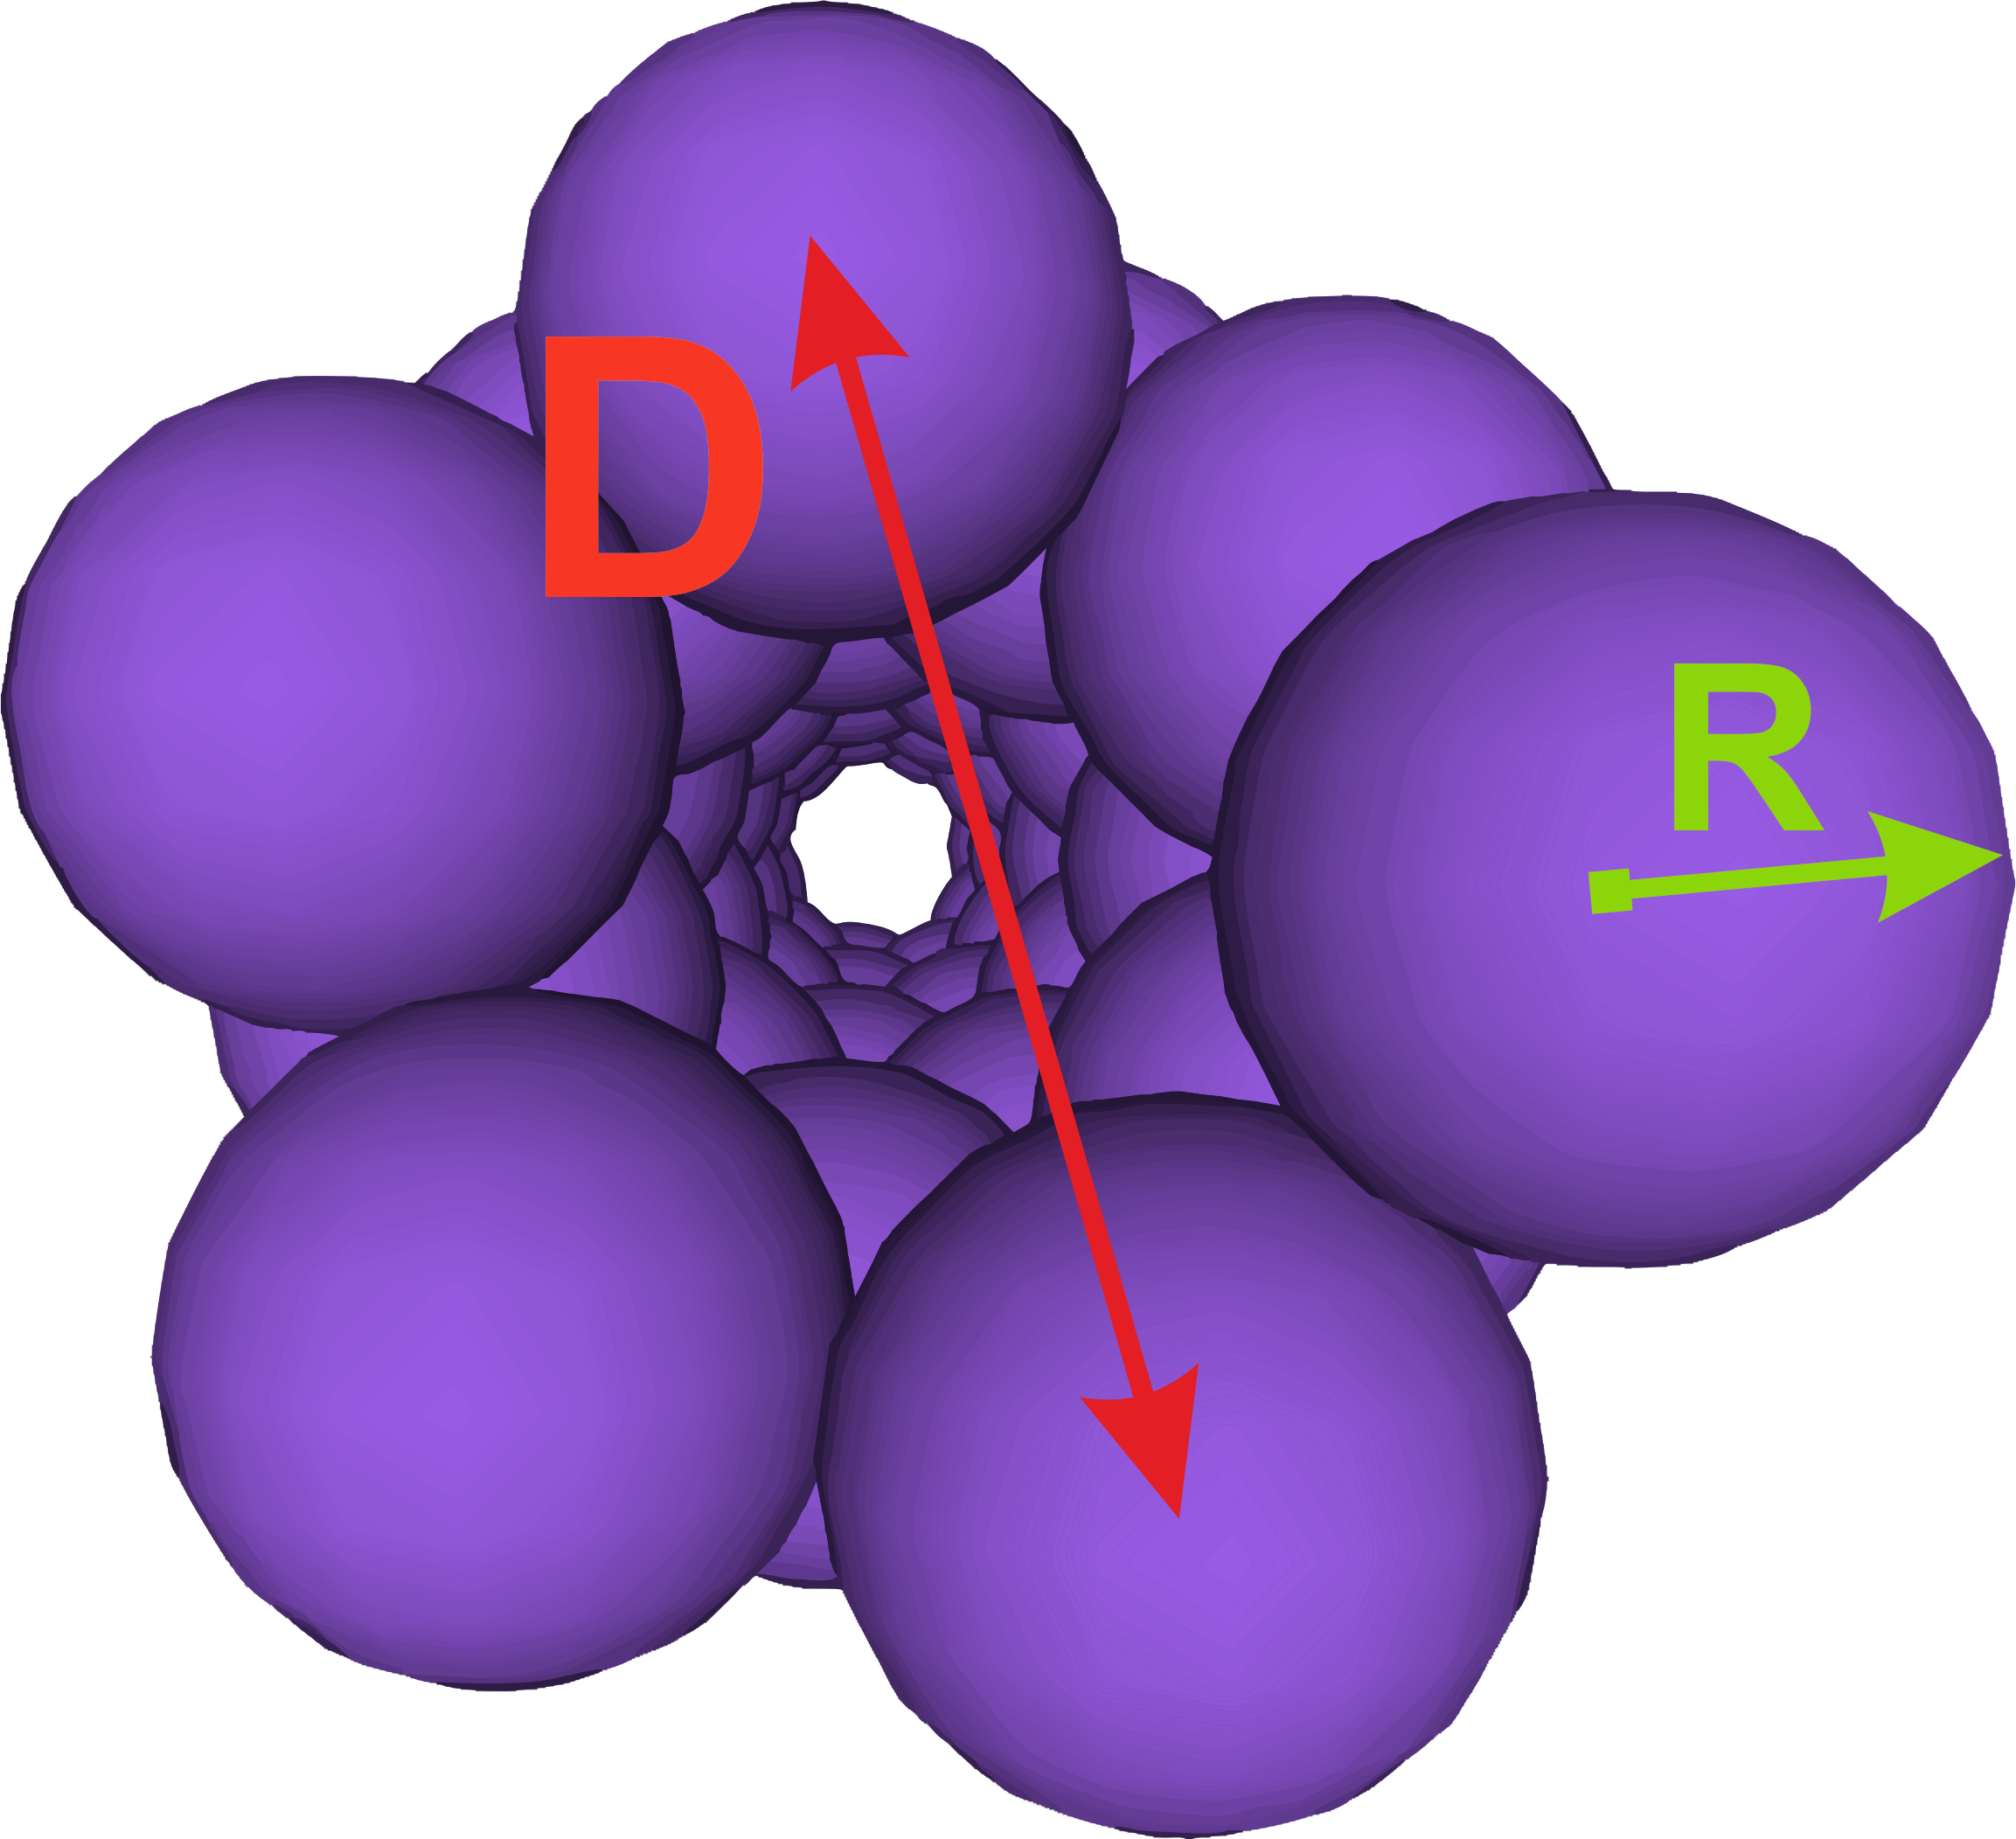
\includegraphics[width=0.4\textwidth]{../images/form_factor/cylindrical_obj/beads_helix_model_2.png}}
%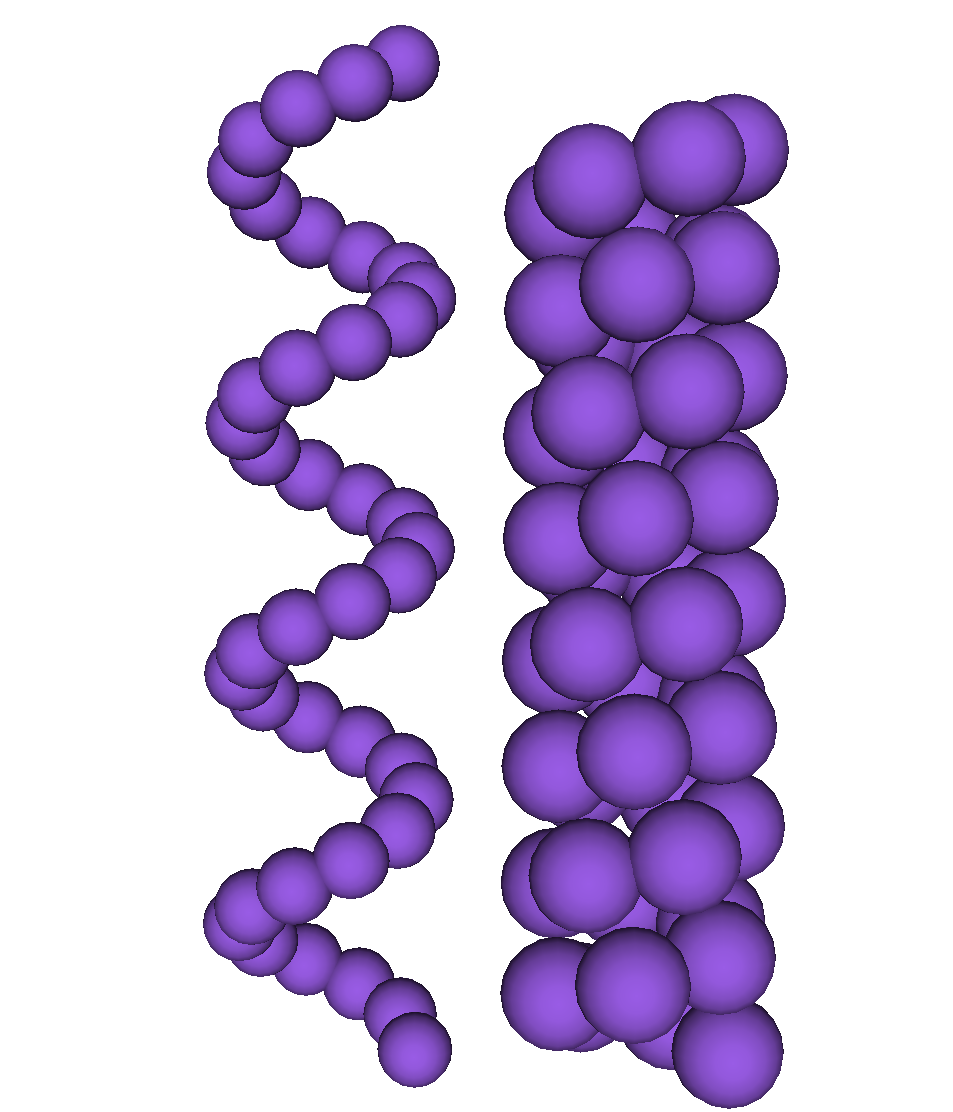
\includegraphics[width=0.4\textwidth,height=0.74\textwidth]{../images/form_factor/cylindrical_obj/beads_helix_model.png}
\end{center}
\caption{Bead model of a helix. In figure a) bead helices with different bead radius and different number of beads per turn are shown} \label{fig:beadshelix}
\end{figure}

\begin{align}
I(Q) &= P_\text{rod}(Q,H) \sum_{j=-\infty}^{\infty} \abs{\frac{nH}{P}\Psi_j\left(QD,\frac{2\pi j}{PQ}\right) \Phi(Q,R)}^2
\label{eq:beadshelix1}
\end{align}
with
\begin{align}
\Psi_j\left(QD,\frac{2\pi j}{PQ}\right) &=
\begin{cases}
\begin{array}{rcl}
J_j\left(\frac{QD}{2}\sqrt{1-\left(\frac{2\pi j}{PQ}\right)}\right) & \text{for} & Q\geq \frac{2\pi\abs{j}}{P}\\
0 & \text{for} & Q < \frac{2\pi\abs{j}}{P}
\end{array}
\end{cases}\\
\Phi(Q,R) &= 3\frac{4\pi}{3}R^3\left(\eta_\text{b}-\eta_\text{solv}\right)\frac{\sin(QR)-QR\cos{QR}}{\left(QR\right)^3} \\
P_\text{rod}(Q,H) &= H^2 \left(2\frac{\mathrm{Si}(QH)}{(QH)}-\left(\frac{\sin(QH/2)}{QH/2}\right)^2\right)
\end{align}
where $\mathrm{Si}(x)=\int_0^x\frac{\sin t}{t}\mathrm{d}t$ is the sine integral. $P_\text{rod}(Q,H)$ is the form factor of an infinitesimal thin rod of length $H$.
$J_j$ is the regular cylindrical Bessel function, for which $J_{j}(x)=(-1)^\abs{j}J_{-j}(x)$ if $j\in \mathbb{Z}$ (integer value) and $j \neq 0$.
Therefore the sum in eq.\ \ref{eq:beadshelix1} can be written as
\begin{align}
I(Q) &= P_\text{rod}(Q,H) \sum_{j=0}^{\infty} \epsilon_j \abs{\frac{nH}{P}\Psi_j\left(QD,\frac{2\pi j}{PQ}\right) \Phi(Q,R)}^2
\label{eq:beadshelix2}
\end{align}
with $\epsilon_j=1$ for $j=0$ and $\epsilon_j=2$ for $j\geq 1$.

The sum converges very fast and for small $Q$-values the first two term are already sufficient. However, {\tt SASfit} is continuing the sum until either the argument below the square root becomes negative or the relative change of the sum is less than $10^{-10}$.

The forward scattering of the model is normalized so that
\begin{align}
I(Q=0) &= \left(H\frac{nH}{P}\frac{4\pi}{3}R^3\left(\eta_\text{b}-\eta_\text{solv}\right)\right)^2
\end{align}

\vspace{5mm}

\underline{Input Parameters for model \texttt{beads helix}:}\\
\begin{description}
\item[\texttt{R}] radius of monomer units/beads $R$
\item[\texttt{D}] mean diameter of helix $D$
\item[\texttt{n}] number of monomer beads per turn $n$
\item[\texttt{dummy}] not used
\item[\texttt{dummy}] not used
\item[\texttt{P}] height of one helix period $P$
\item[\texttt{H}] total length of helix $H$
\item[\texttt{eta\_b}] scattering length density of monomer beads $\eta_\text{b}$
\item[\texttt{dummy}] not used
\item[\texttt{eta\_solv}] scattering length density of solvent $\eta_\text{solv}$
\end{description}

\noindent\underline{Note:}
\begin{itemize}
\item The helix is assumed to be stiff and long so that it scattering intensity can be factorized in a cross-section contribution and a shape contribution, whereas the shape contribution can be described by an infinitesimal thin rod of length $H$.
\item $R$, $P$, $D$, $H$, and $n$ are only physical for values larger than 0.
\item The model is an approximation for the limit $H \gg P$ and $H \gg D$.
\end{itemize}

\begin{figure}[htb]
\begin{center}
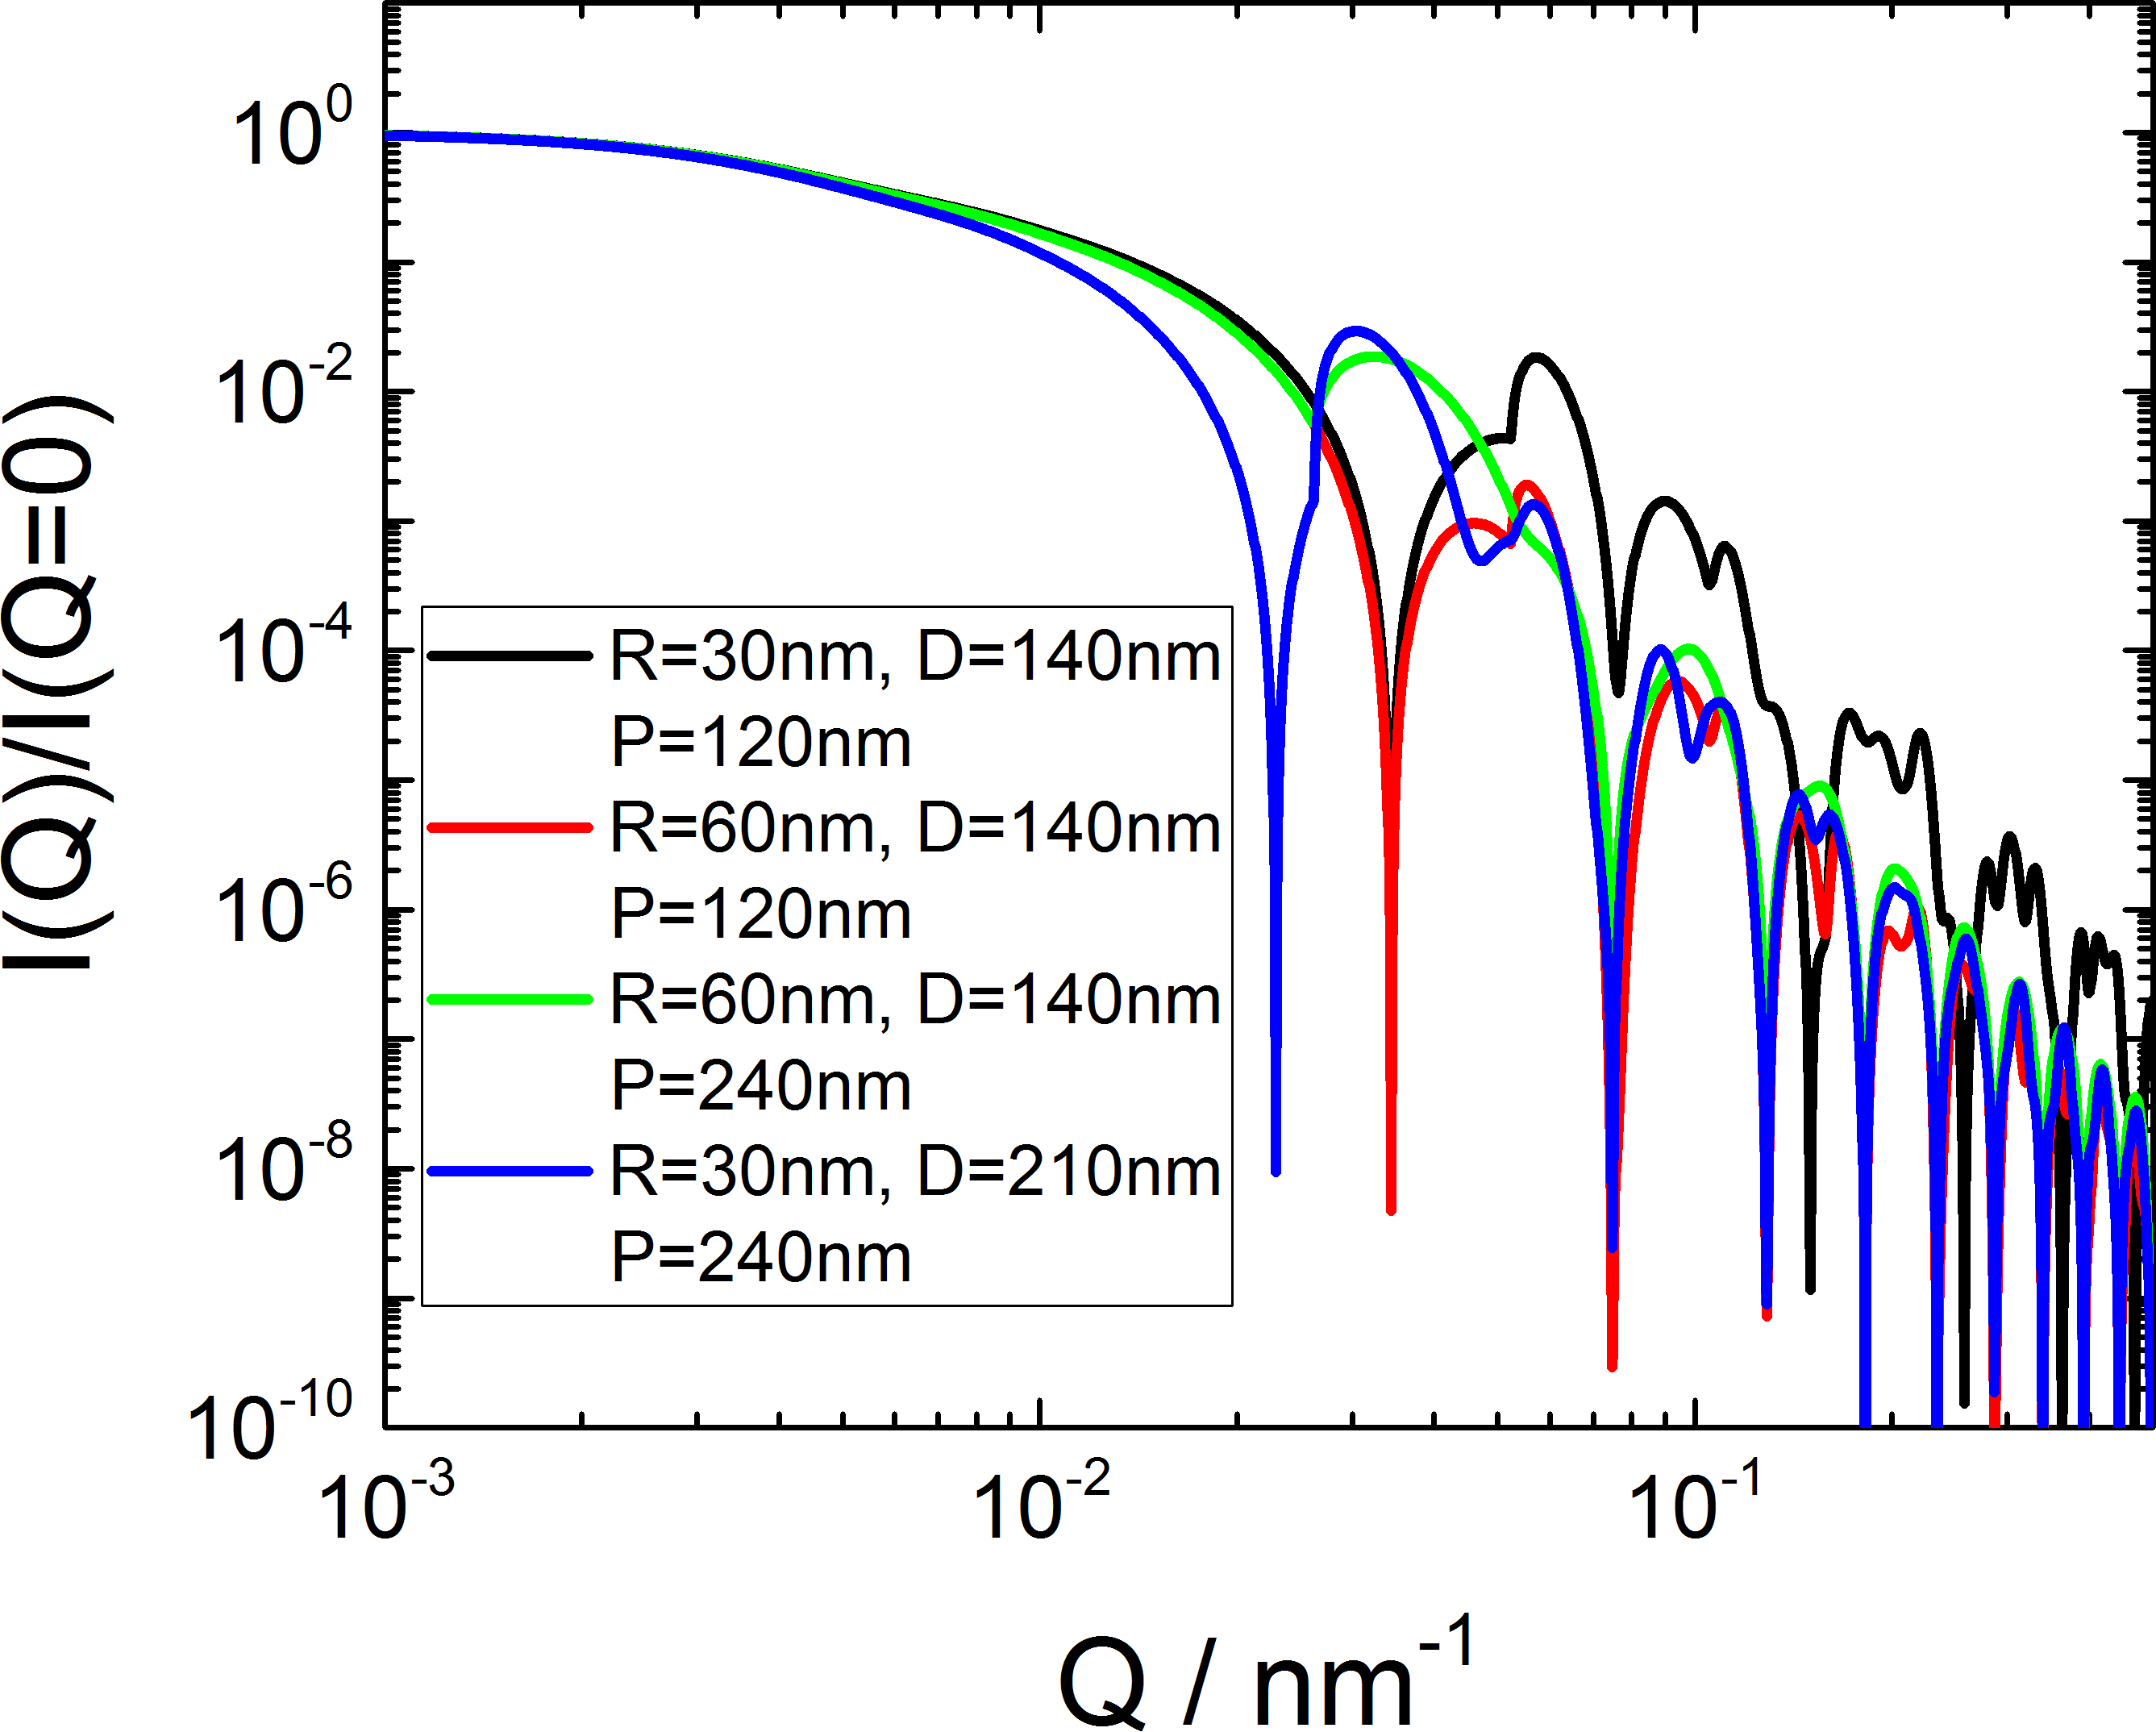
\includegraphics[width=0.7\textwidth]{../images/form_factor/cylindrical_obj/helix_beadsIQ.png}
\end{center}
\caption{Normalized scattering curves of a single stranded helices formed by spherical beads.}
\label{fig:helixbeadsIQ}
\end{figure}


%\phantom{.}~\\
\newpage
\subsubsection{straight superhelix} ~\\
Benham et al.\ \cite{Benham1980} and Crick \cite{Crick1953} describe single helices with a secondary helical curvature, which they call coiled superhelices or coiled coil. They assume in their analysis an infinitesimal thin helical strand.
\begin{figure}[htb]
\begin{center}
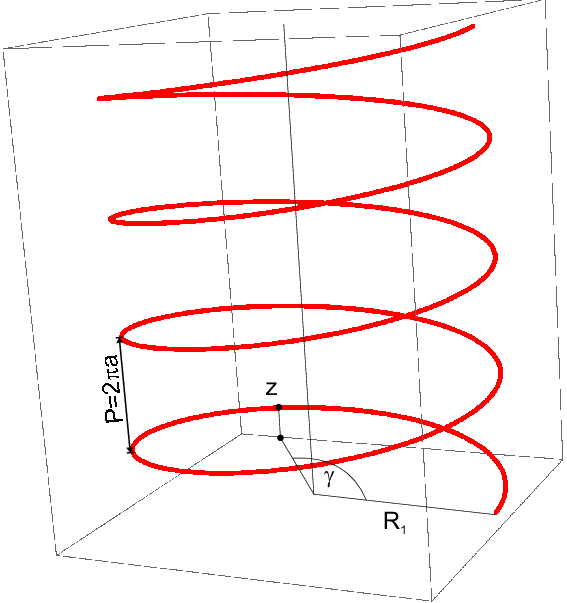
\includegraphics[width=0.497\textwidth,height=0.529\textwidth]{../images/form_factor/cylindrical_obj/straightSuperhelix.png}
\end{center}
\caption{infinitesimal thin single stranded helix} \label{fig:straightsuperhelix}
\end{figure}
 The straight superhelix is their starting geometry without a secondary coiling. The expression for a random oriented straight superhelix of finite length can be written exact in form of a single integral and is given by
\begin{align}
I(Q) &= 2 \int_0^{\mathcal{L}} \frac{(\mathcal{L}-w)\sin Q\psi}{Q\psi} \mathrm{d}w \\
\psi &= + \sqrt{2 R_1^2\left[1-\cos\left(\frac{w}{\sqrt{R_1^2+a^2)}}\right) \right]+\frac{a^2w^2}{R_1^2+a^2}} \\
\mathcal{L} &= 2\pi \frac{H}{P} \sqrt{R_1^2+a^2} \\
a &= \frac{P}{2\pi}
\end{align}
$\mathcal{L}$ is the arclength of the helix, $R_1$ the distance to the helix axis and $P$ the pitch of the helix. The intensity is normalized to the squared arclength of the helix. i.e.
\begin{align}
I(Q=0)&=\mathcal{L}^2
\end{align}

\vspace{5mm}

\underline{Input Parameters for model \texttt{straight superhelix}:}\\
\begin{description}
\item[\texttt{R\_1}] distance to the helix axis $R_1$
\item[\texttt{dummy}] not used
\item[\texttt{dummy}] not used
\item[\texttt{dummy}] not used
\item[\texttt{dummy}] not used
\item[\texttt{P}] height of one helix period $P$
\item[\texttt{H}] total length of helix $H$
\item[\texttt{dummy}] not used
\item[\texttt{dummy}] not used
\item[\texttt{dummy}] not used
\end{description}

\noindent\underline{Note:}
\begin{itemize}
\item the model assumes an infinitesimal thin single helical strand.
\item $R_1$, $P$, and $H$ are only physical for values larger than 0.
\item The model is exact.
\end{itemize}

\begin{figure}[htb]
\begin{center}
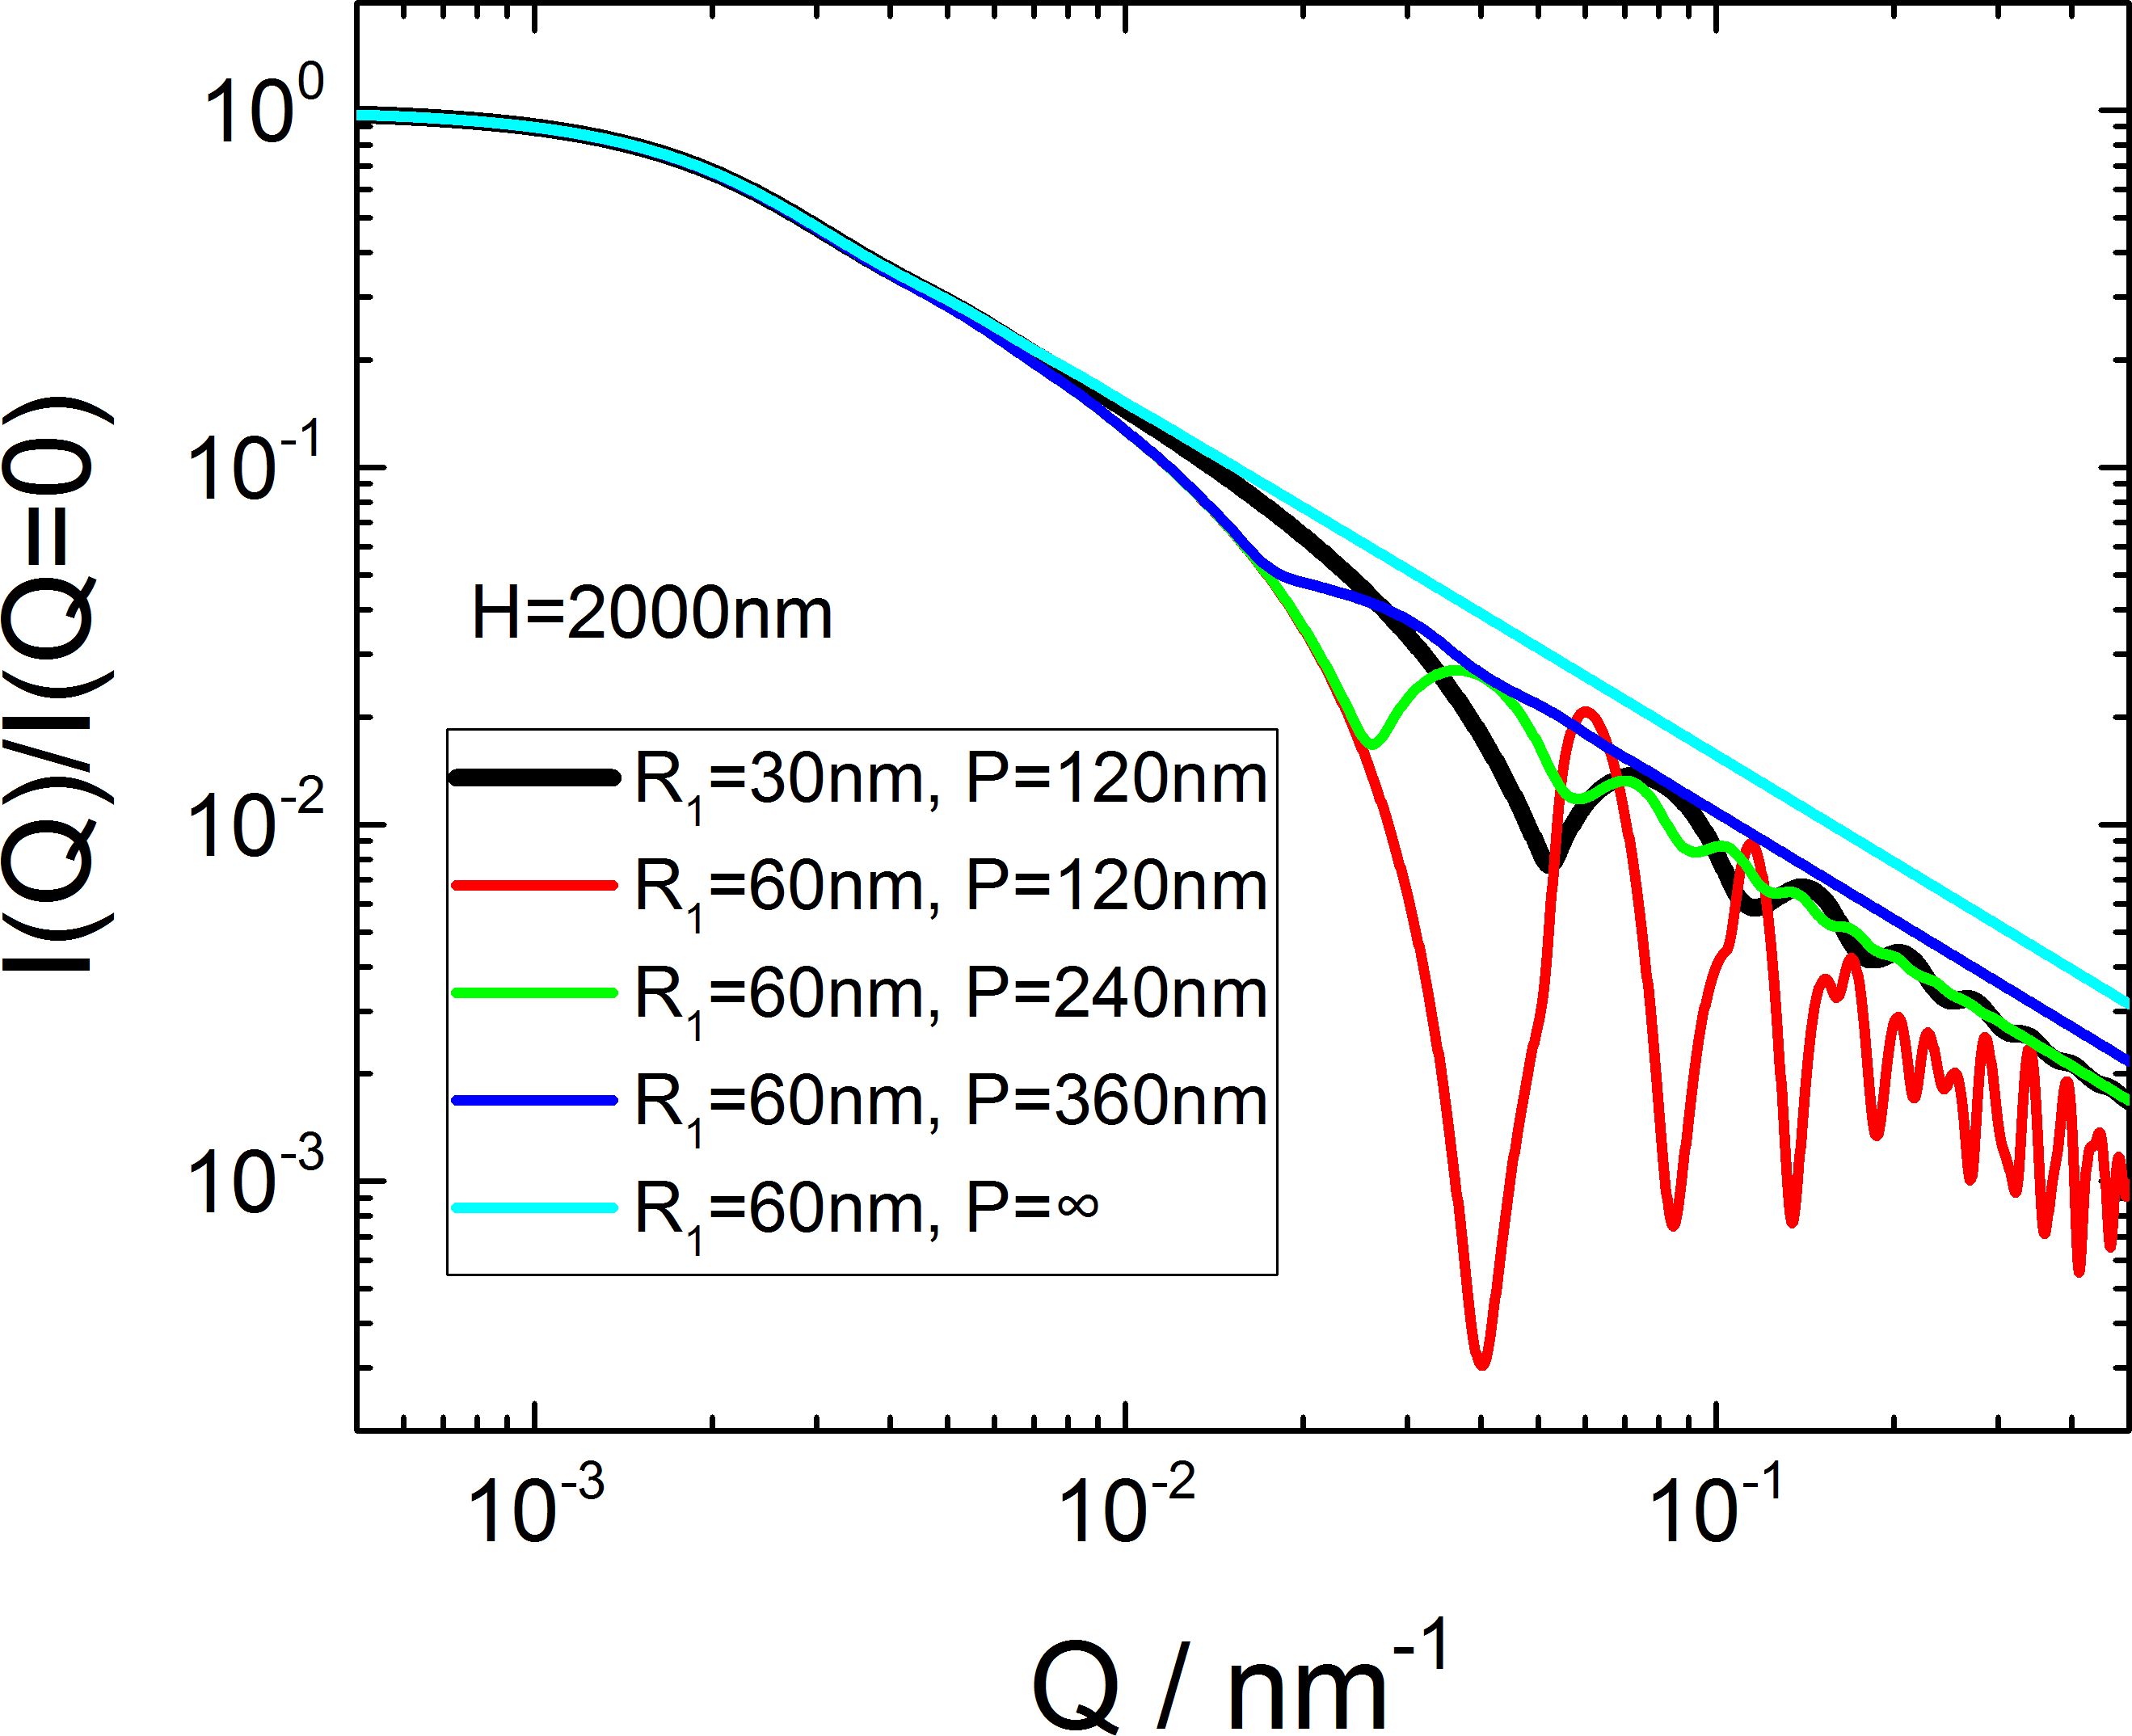
\includegraphics[width=0.7\textwidth]{../images/form_factor/cylindrical_obj/helix_straightIQ.png}
\end{center}
\caption{Normalized scattering curves of single stranded infinitesimal thin stranded helices.}
\label{fig:helixstraightIQ}
\end{figure}

%\phantom{.}~\\
\newpage
\subsubsection{coiled superhelix} ~\\
A coiled superhelix or coiled coil is a helix with a small repeat whose axis is slightly deformed and follows a larger more graded helical path \cite{Benham1980,Crick1953}.
\begin{figure}[htb]
\begin{center}
  \subfigure[A superhelix with primary and secondary turns. The bottom one has ten times more primary turns per secondary turn than the top one]{\label{fig:superhelixcoiled1}
  \begin{minipage}[b]{0.45\textwidth}
  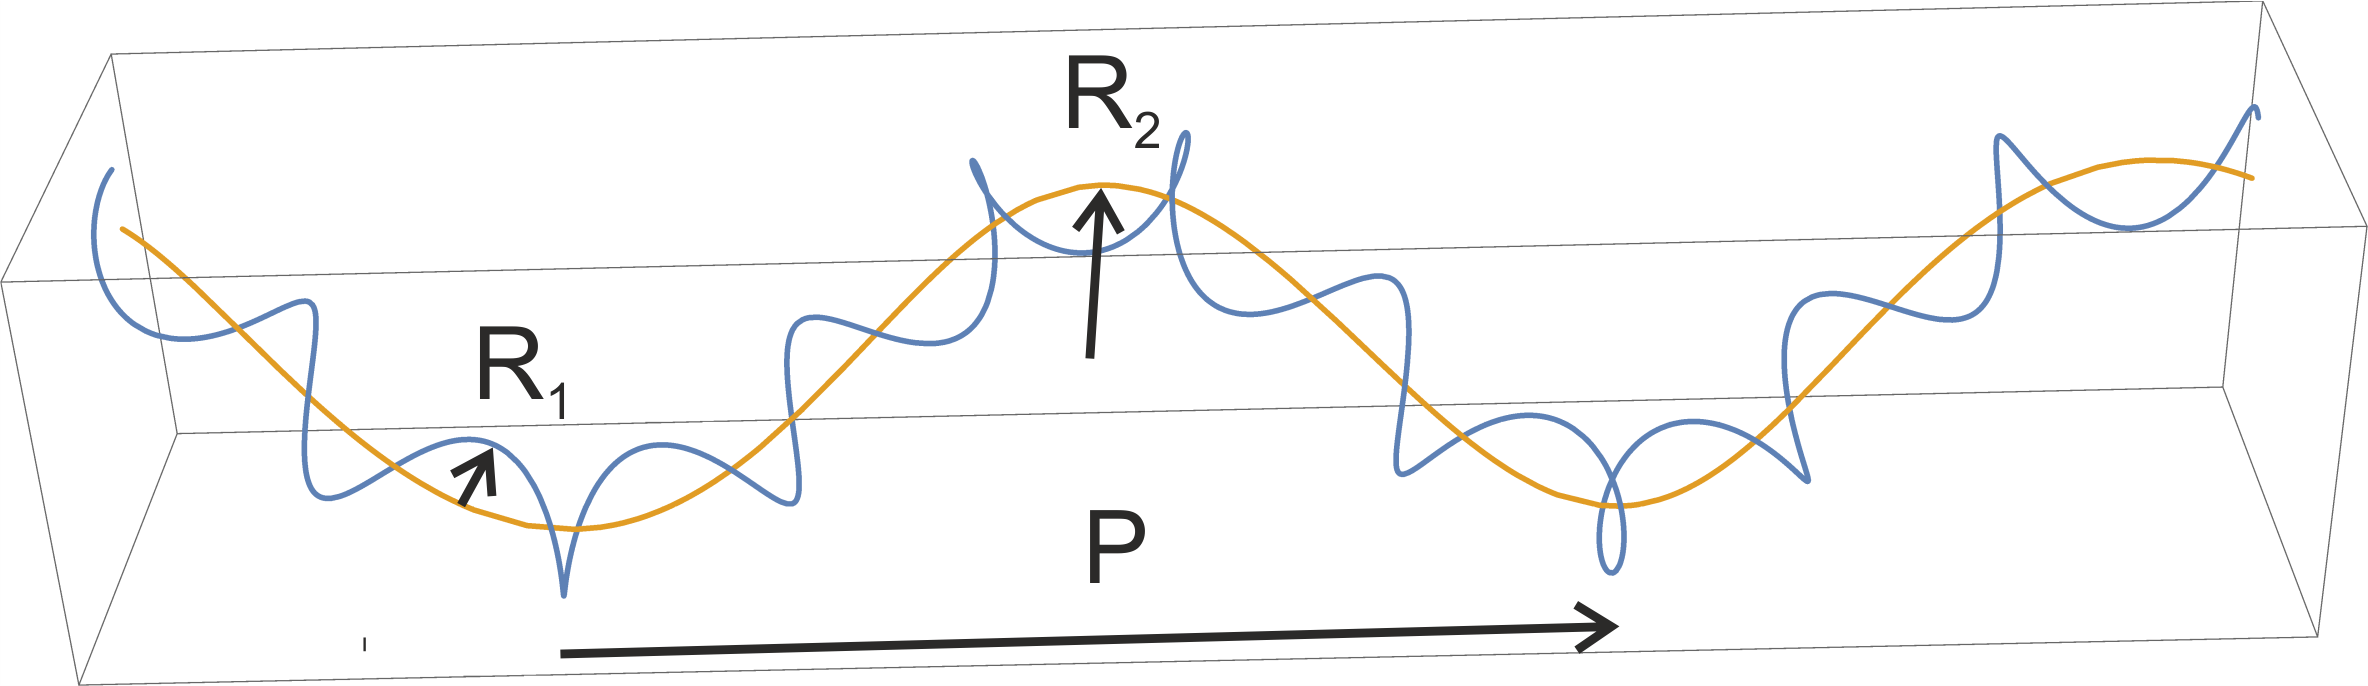
\includegraphics[width=\textwidth]{../images/form_factor/cylindrical_obj/superhelixcoiled1.png} \\
  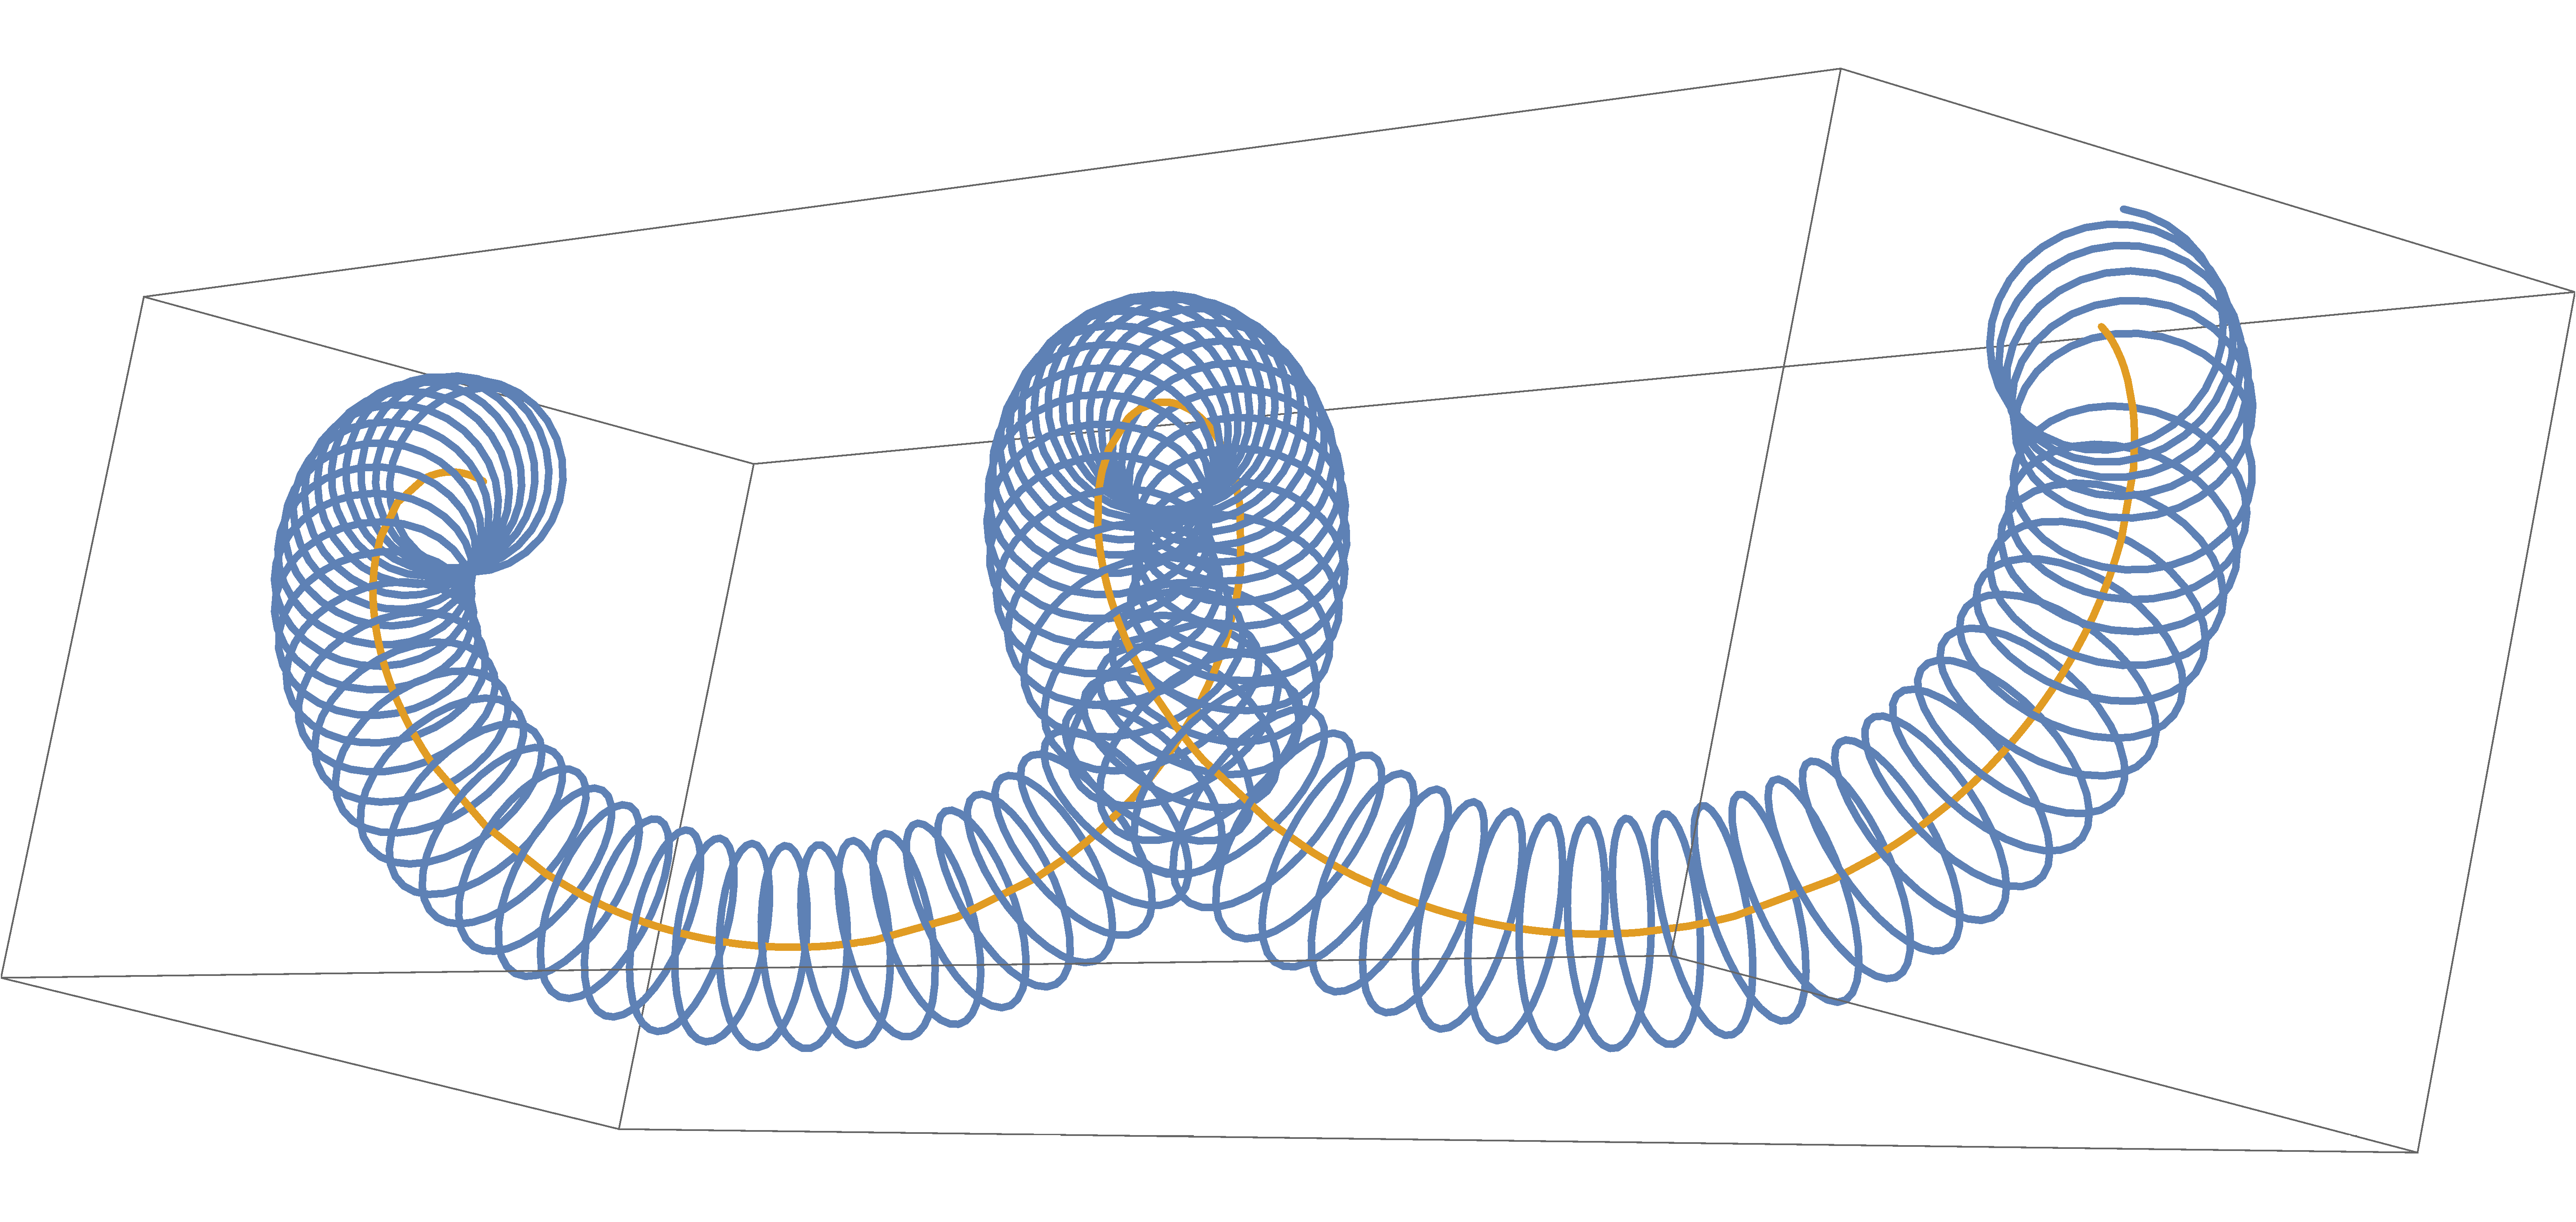
\includegraphics[width=\textwidth]{../images/form_factor/cylindrical_obj/superhelixcoiled2.png}
  \end{minipage}
  }
\hfill
  \subfigure[A superhelix with zero pitch forms a toroidal helix]{\label{fig:superhelixcoiled2}
  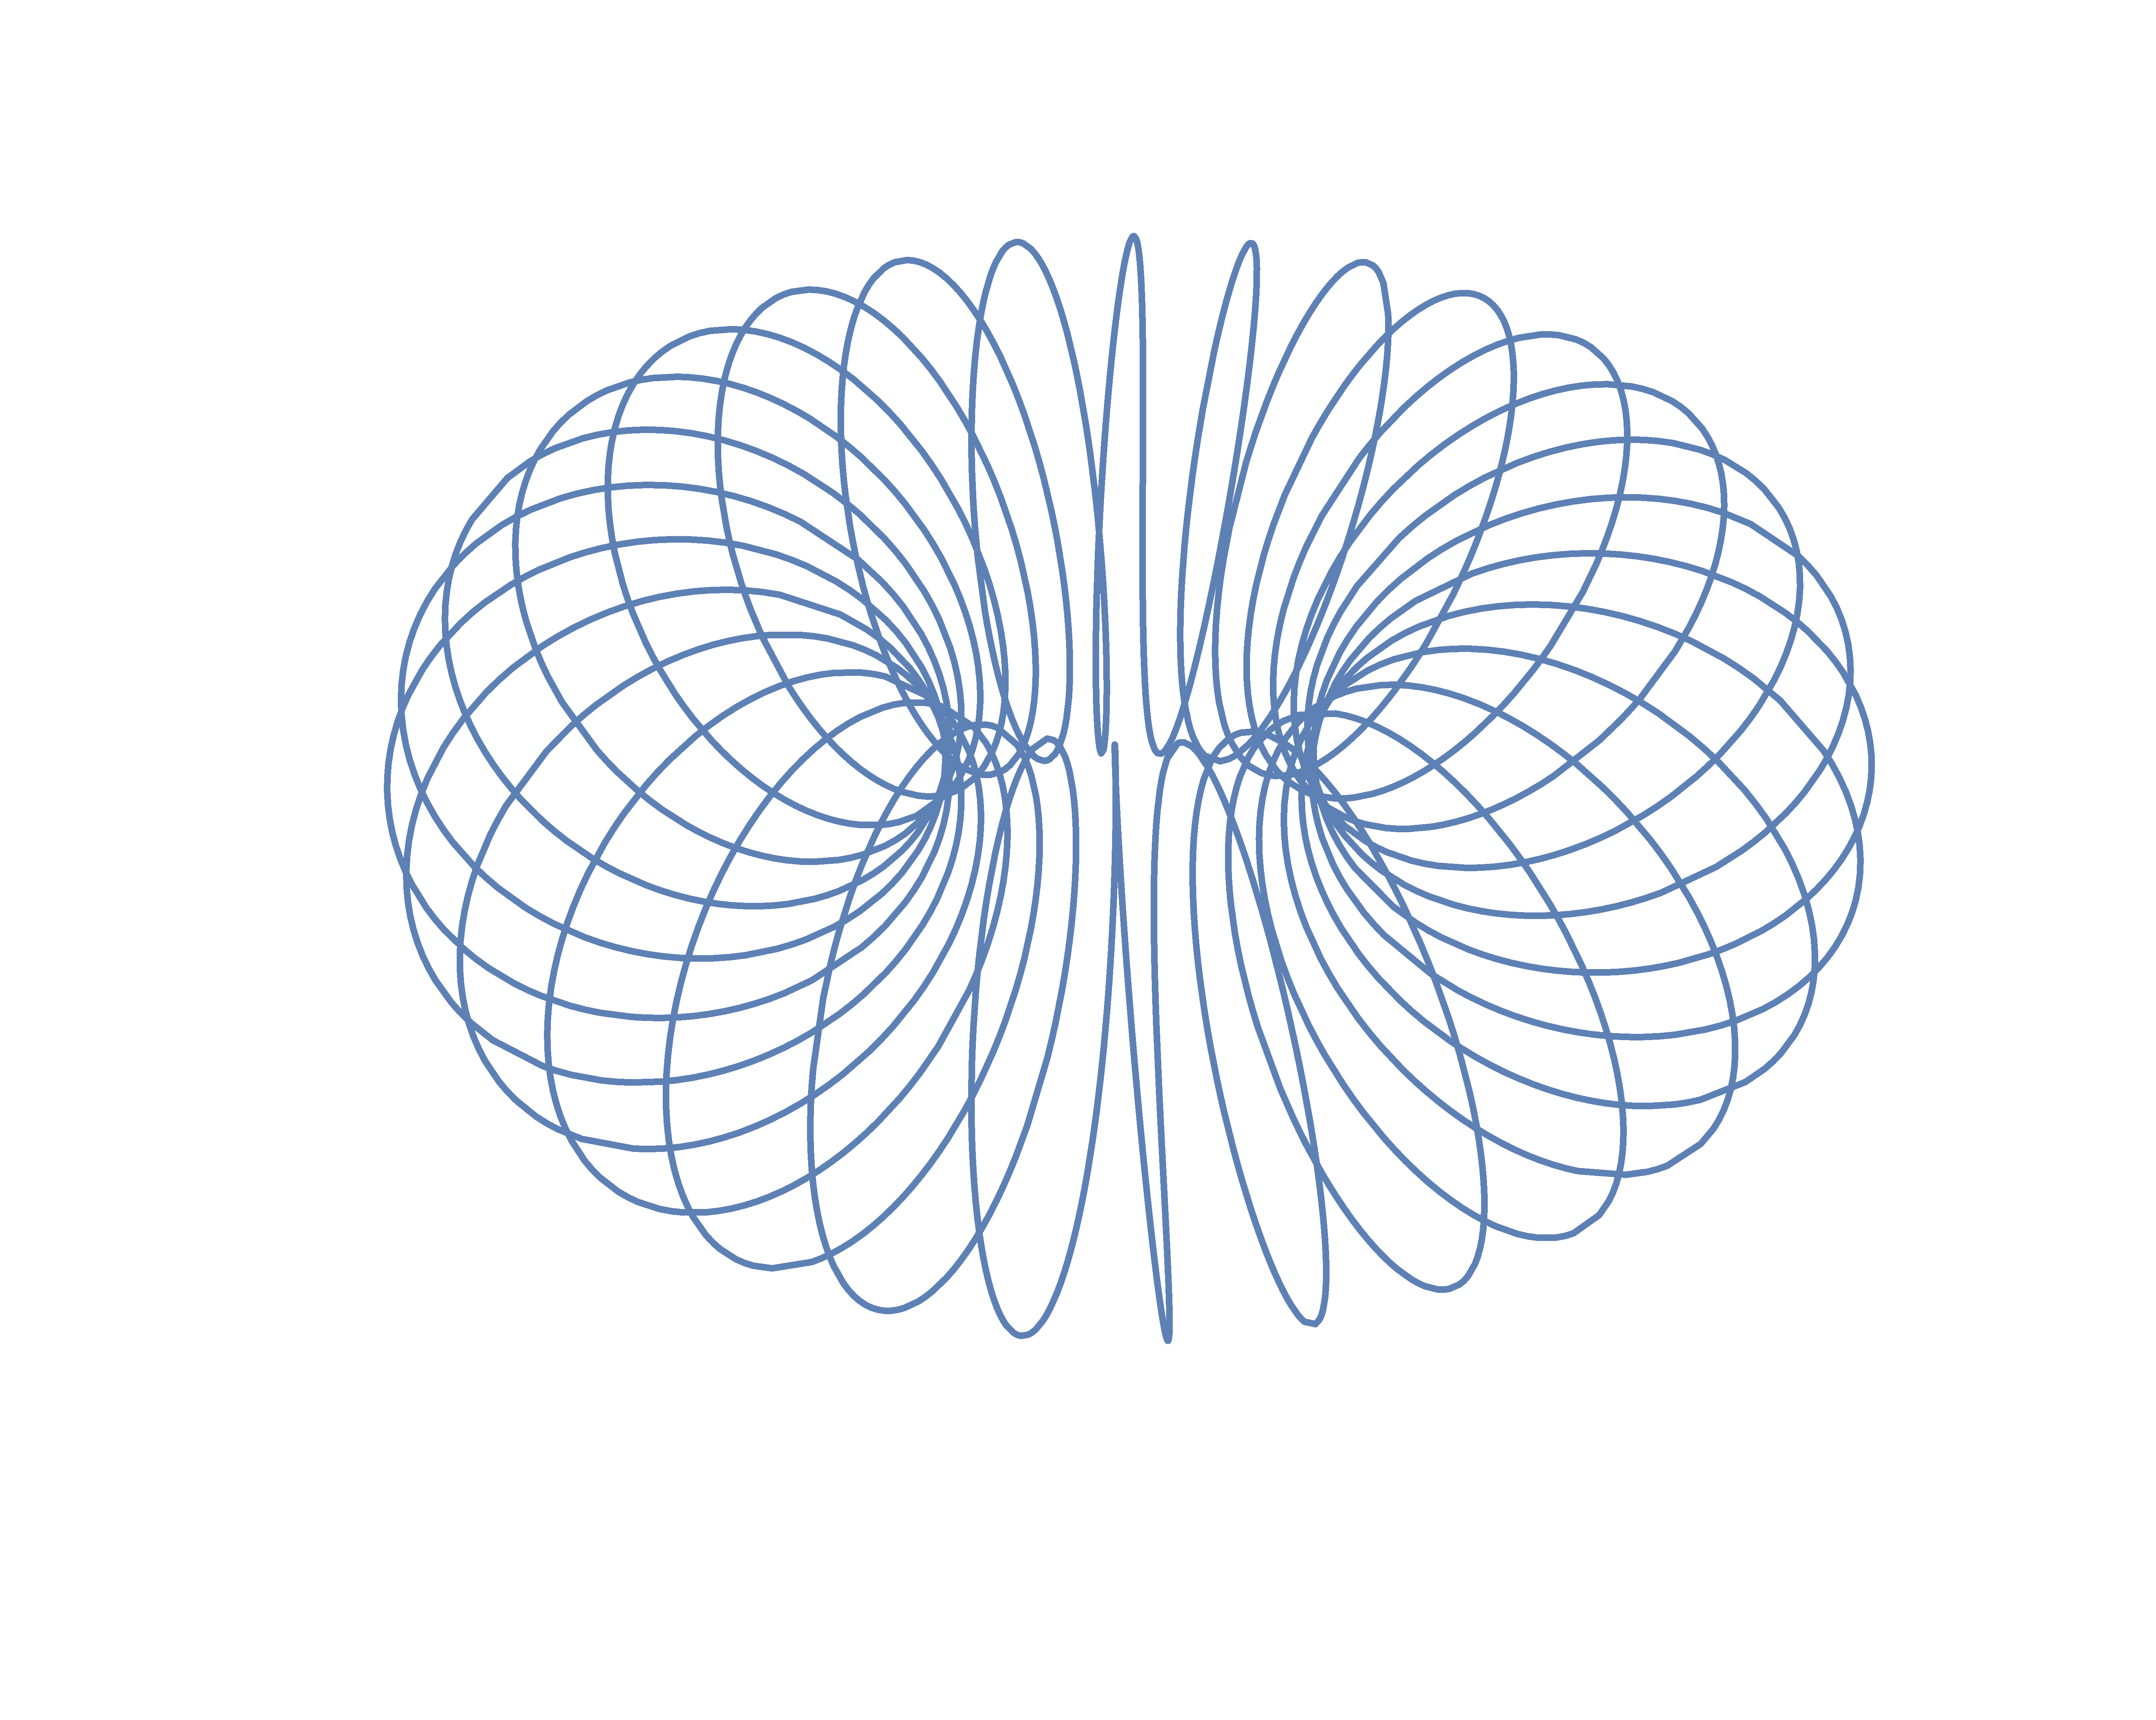
\includegraphics[width=0.45\textwidth]{../images/form_factor/cylindrical_obj/superhelixcoiled3.png}
  }
\end{center}
\caption{Combinations of two helical orders are
referred to as coiled coils or coiled superhelix.} \label{fig:superhelixcoiled}
\end{figure}


The points $p(\gamma)=\left[x(\gamma),y(\gamma),z(\gamma)\right]$ on the coiled superhelix are parametrized by
\begin{align}
x(\gamma) &= \cos\left(\gamma\right) \left(R_2+R_1\cos\left(N\gamma\right)\right)
            - R_1\cos\left(\alpha_2\right)\sin\left(\gamma\right)\sin\left(N\gamma\right) \\
y(\gamma) &= \sin\left(\gamma\right) \left(R_2+R_1\cos\left(N\gamma\right)\right)
            - R_1\cos\left(\gamma\right)\sin\left(N\gamma\right)\cos\left(\alpha_2\right) \\
z(\gamma) &= \frac{P}{2\pi}\gamma - R_1\sin\left(\alpha_2\right)\sin\left(N\gamma\right)
\end{align}
$R_1$ and $R_2$ are the radii of the primary and secondary coiling of the superhelix. $P$ is the pitch of the secondary coiling and $\alpha_2= \arctan\left(\frac{2\pi R_2}{P}\right)$ its pitch angle. $N$ is the number of first order tuns in the primary coiling for each turn of the secondary coiling.
The arc length of the helix $\mathcal{L}$ can be calculated by
\begin{align}
\mathcal{L} &= \int_0^{\gamma_\mathrm{max}} \sqrt{f(\gamma)} \mathrm{d}\gamma
\end{align}
with
\begin{align}
\begin{split}
f(\gamma) &= R_2^2+R_1^2N^2 \left(\cos^2\left(N\gamma\right)+\sin^2\left(N\gamma\right)\cos^2(\alpha_2)\right) \\
&+\frac{P^2}{(2\pi)^2} + 2R_2*R_1\cos\left(N\gamma\right) +2R_1^2N\cos(\alpha_2)
\end{split}
\end{align}
and
\begin{align}
\gamma_\mathrm{max} &= N_\mathrm{2nd}/(2\pi)
\end{align}
where $N_\mathrm{2nd}$ is the number of secondary turns of the coiled superhelix.
The scattering intensity is than given by
\begin{align}
I(Q) &= \int_0^{\gamma_\mathrm{max}} \mathrm{d}\gamma_2 \int_0^{\gamma_\mathrm{max}} \sqrt{f(\gamma_2)f(\gamma_1)}
\frac{\sin\left( Qr(\gamma_1,\gamma_2)\right)}{Qr(\gamma_1,\gamma_2)} \mathrm{d}\gamma_2
\end{align}
with
\begin{align}
r^2(\gamma_1,\gamma_2) &= \left( \begin{pmatrix}
                            x(\gamma_2) \\
                            y(\gamma_2) \\
                            z(\gamma_2) \\
                          \end{pmatrix}
                        - \begin{pmatrix}
                            x(\gamma_1) \\
                            y(\gamma_1) \\
                            z(\gamma_1) \\
                          \end{pmatrix} \right)^2
\end{align}
The intensity is normalized to the squared arclength of the helix. i.e.
\begin{align}
I(Q=0)&=\mathcal{L}^2
\end{align}

\vspace{5mm}

\underline{Input Parameters for model \texttt{coiled superhelix}:}\\
\begin{description}
\item[\texttt{R\_1}] distance to the primary helix axis $R_1$
\item[\texttt{R\_2}] distance to the primary helix axis $R_1$
\item[\texttt{dummy}] not used
\item[\texttt{N}] number of primary turns $N$ per secondary turn
\item[\texttt{dummy}] not used
\item[\texttt{P}] pitch length of secondary helix $P$
\item[\texttt{turns}] number of secondary turns $N_\mathrm{2nd}$
\item[\texttt{dummy}] not used
\item[\texttt{dummy}] not used
\item[\texttt{dummy}] not used
\end{description}

\noindent\underline{Note:}
\begin{itemize}
\item the model assumes an infinitesimal thin single helical strand with an additional secondary coiling.
\item $R_1$,$R_2$, $P$, $N_\mathrm{2nd}$ and $N$ are only physical for values larger than 0.
\item The model is exact.
\item The calculation of the scattering intensity requires a double integration, which is the reason for the longer computing time.
\end{itemize}

\begin{figure}[htb]
\begin{center}
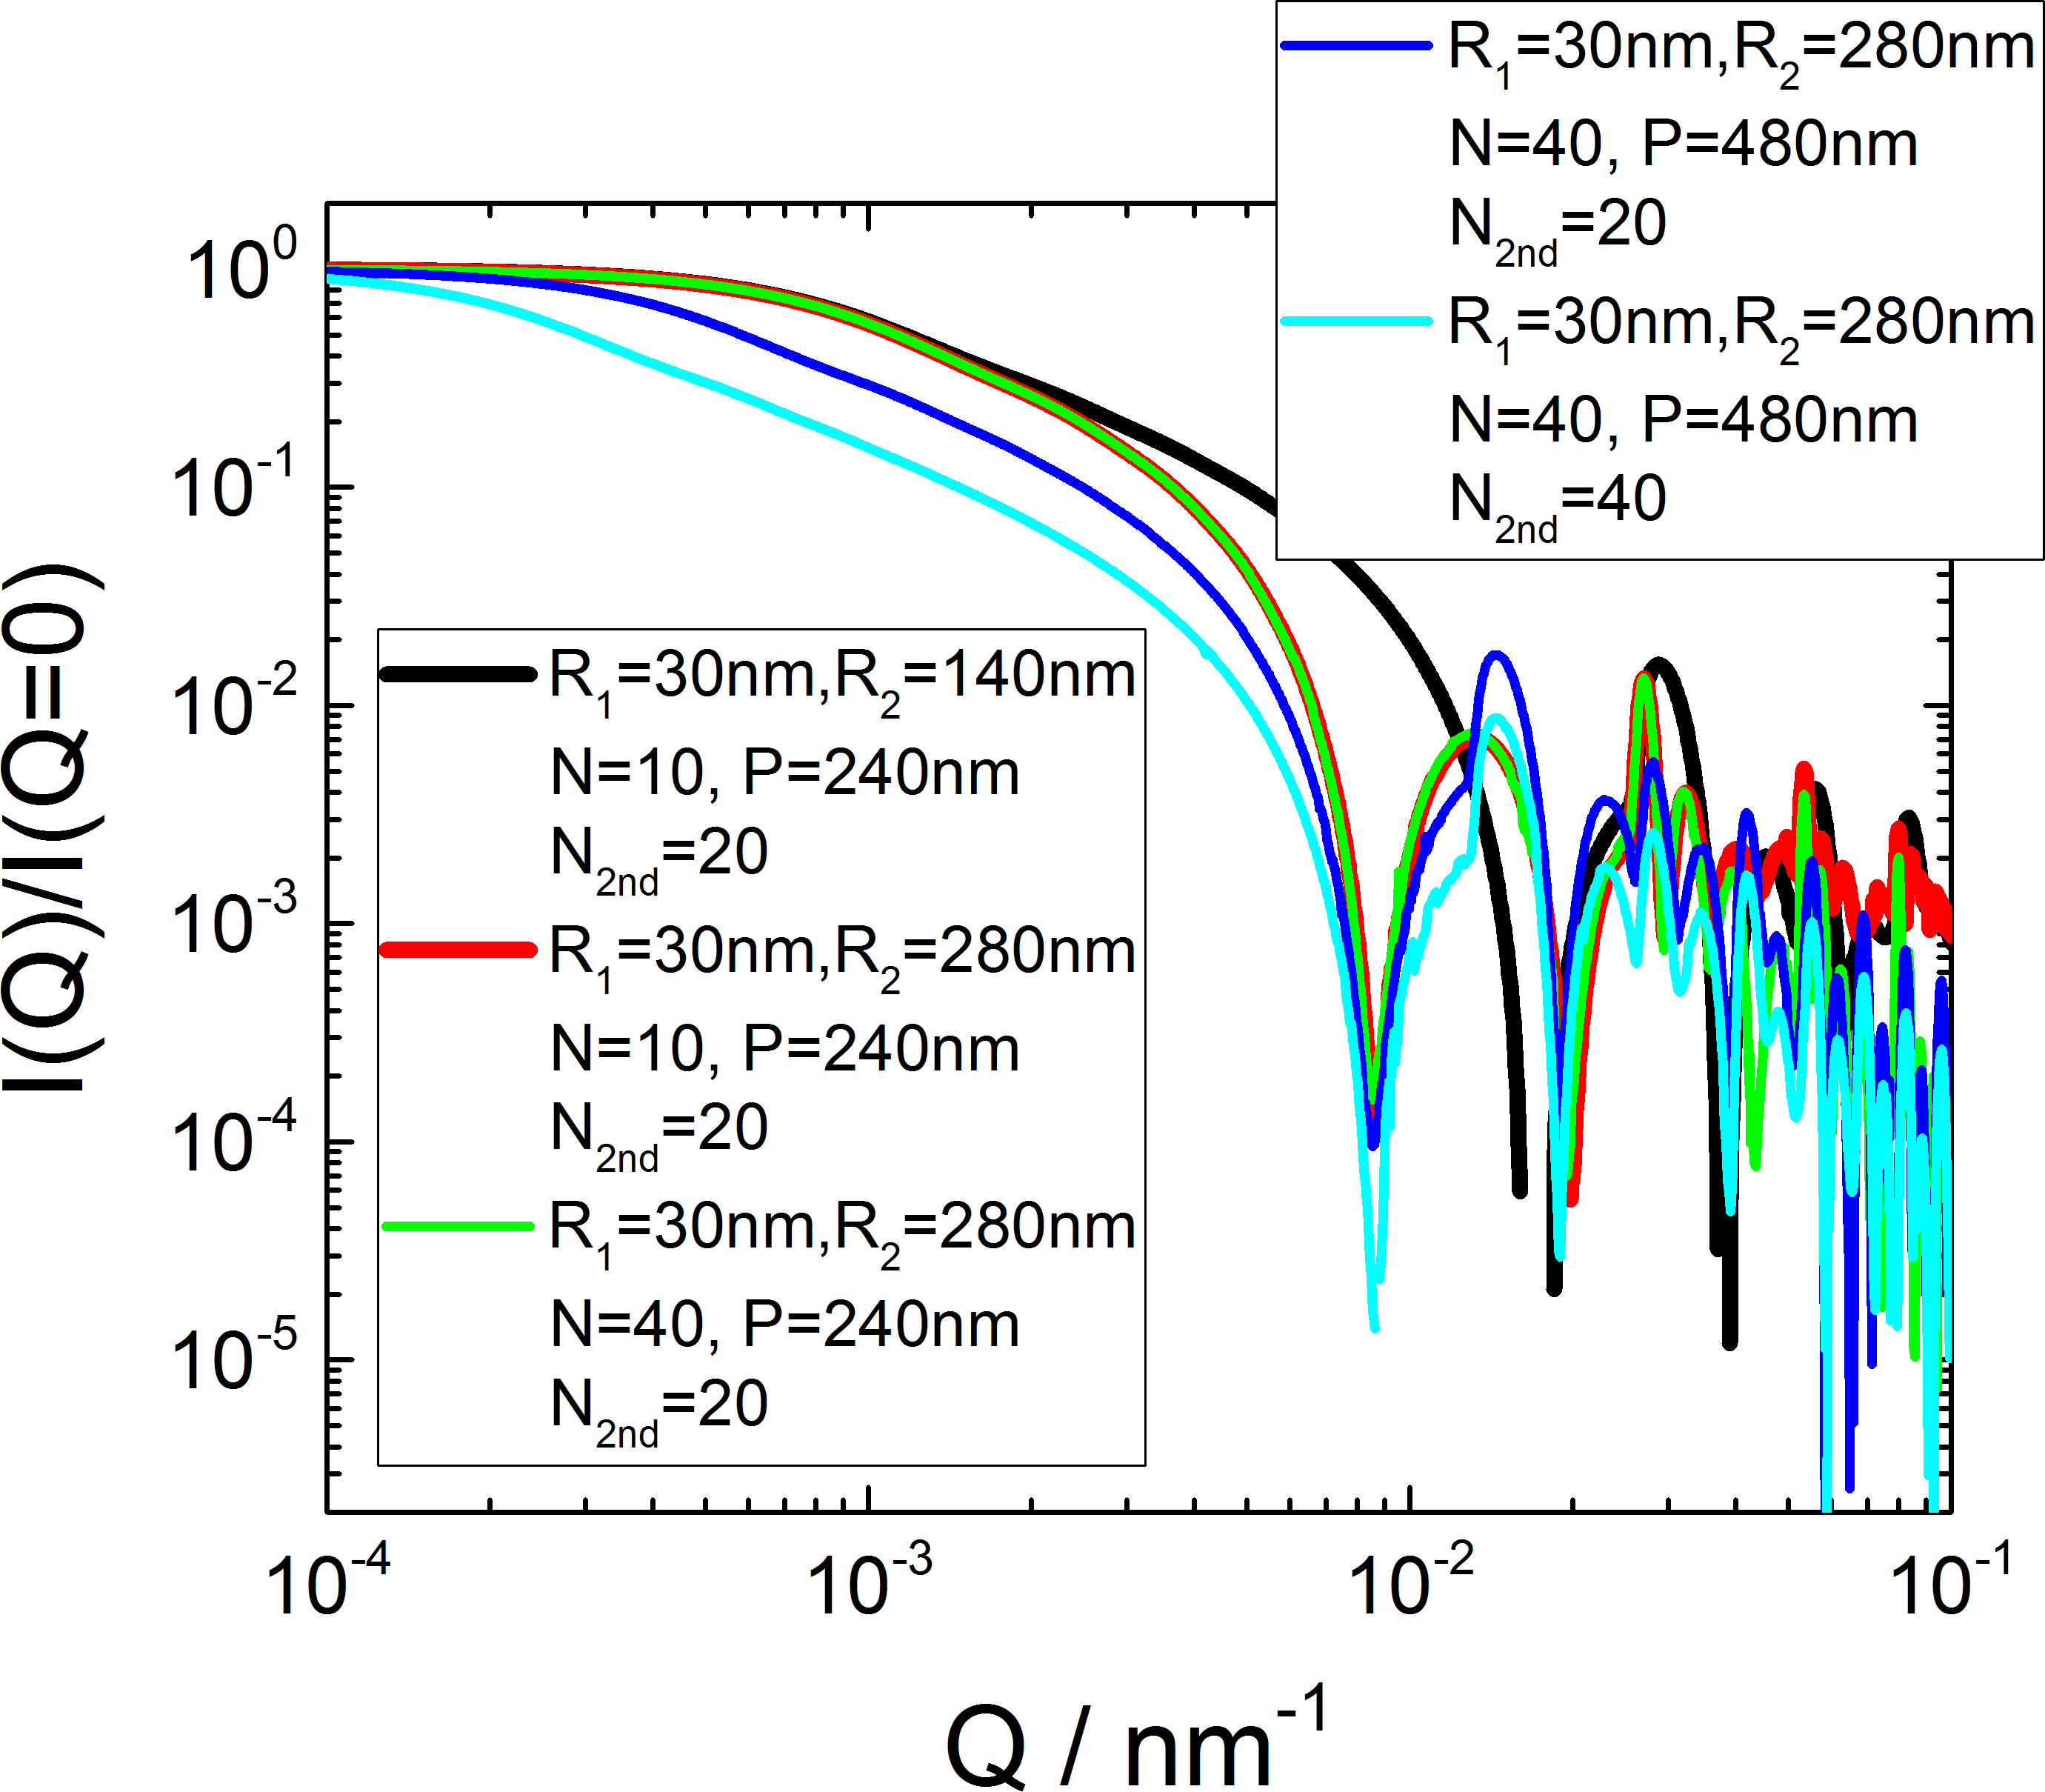
\includegraphics[width=0.7\textwidth]{../images/form_factor/cylindrical_obj/helix_coiledIQ.png}
\end{center}
\caption{Normalized scattering curves of single stranded infinitesimal thin coiled helices.}
\label{fig:helixcoiledIQ}
\end{figure} 